\documentclass[abstract=on,10pt,a4paper,bibliography=totocnumbered]{article}
\usepackage[paper=a4paper,left=35mm,right=35mm,top=25mm,bottom=30mm]{geometry}
\usepackage[doublespacing]{setspace}
\usepackage[english]{babel}
\usepackage[utf8]{inputenc}
\usepackage[round]{natbib}
\usepackage{amsmath}
\usepackage{colortbl}
\usepackage{amsfonts}
\usepackage{amssymb}
\usepackage{gensymb}
\usepackage{graphicx}
\usepackage{tikz}
\usepackage{enumerate}
\usepackage{enumitem}
\usepackage{subcaption}
\usepackage{booktabs}
\usepackage[hidelinks]{hyperref}
\usepackage[nameinlink]{cleveref}
\usepackage{lineno}
\usepackage{multirow}
\usepackage{arydshln}
\usepackage[flushleft]{threeparttable}
\usepackage[nomarkers, nolists]{endfloat}

%------------------------------------------------------------------------------
%	Some Styling
%------------------------------------------------------------------------------
% Creating some TikZ styles
\tikzset{
  nonterminal/.style = {rectangle
    , minimum size = 6mm
    , very thick
    , draw = black!
  }
}

% Changing the style of captions in figures etc.
\captionsetup{labelfont=bf, format=plain, font=small}

% Change how equations are referenced
\renewcommand{\theequation}{Equation \arabic{equation}}%

%------------------------------------------------------------------------------
%	Titlepage: Header
%------------------------------------------------------------------------------
\title{Step by Step: Using Step Selection Functions to Simulate Dispersal and
Assess Landscape Connectivity}

% \title{Step by Step: The Utility of Dispersal Simulations to Assess Landscape
% Connectivity}

% List of Authors
\author{
  David D. Hofmann\textsuperscript{1,\S} \and
  John W. McNutt\textsuperscript{2} \and
  Arpat Ozgul\textsuperscript{1} \and
  Gabriele Cozzi\textsuperscript{1,2} \and
  Dominik M. Behr\textsuperscript{1,2}
}

% Reduce spacing between authors
\makeatletter
\def\and{%
  \end{tabular}%
  \hskip -0.5em \@plus.17fil\relax
  \begin{tabular}[t]{c}}
\makeatother

% Current Date
\date{\today}

% And here the masterpiece begins
\begin{document}

% Change page numbering
\pagenumbering{gobble}

% Required to be able to cite
\bibliographystyle{apalike}

% Create Titlepage
\maketitle

%------------------------------------------------------------------------------
%	Titlepage: Additional Info
%------------------------------------------------------------------------------
\begin{flushleft}

\vspace{0.5cm}

\textsuperscript{1} Department of Evolutionary Biology and Environmental
Studies, University of Zurich, Winterthurerstarsse 190, 8057 Zurich,
Switzerland.

\textsuperscript{2} Botswana Predator Conservation, Private Bag 13, Maun,
Botswana.

\textsuperscript{\S} Corresponding author (david.hofmann2@uzh.ch)

\vspace{4cm}

\textbf{Running Title:} Release the Dogs! Simulating Wild Dog Dispersal to
Assess Landscape Connectivity

\vspace{0.5cm}

\textbf{Keywords:} dispersal, simulation, movement, integrated step selection,
Kavango-Zambezi Transfrontier Conservation Area, landscape connectivity, Lycaon
pictus

\end{flushleft}

%------------------------------------------------------------------------------
%	Abstract
%------------------------------------------------------------------------------
\newpage
\begin{abstract}
Dispersal is an important process that allows species to avoid inbreeding, to
colonize new habitats and to reinforce non-viable subpopulations. Successful
dispersal thus represents a crucial pre-requisite for long-term species
persistence in wild animal populations. However, the ability to disperse is
contingent a sufficient degree of landscape connectivity, which is why the
estimation of connectivity and identification of dispersal corridors has become
a task of extraordinary importance for conservation authorities worldwide.

Over the past two decades, ecologists have primarily relied on analytical tools
such as least-cost analysis and circuit theory to model and investigate
landscape connectivity. Despite their usefulness for a diverse suite of
ecological applications, both methods make several restricting assumptions that
limit their suitability in reality. To address these shortcomings, dispersal
simulations from individual-based movement models have been proposed and
applied. Yet, due to the almost infinite amount of non-trivial decisions a
modeler faces when parametrizing such models, a unified and objective framework
is missing.

Recent innovations in movement ecology have brought forward novel opportunities
to study animal dispersal and estimate landscape connectivity. In particular,
the rich suite of resource selection functions, namely point-, step-, and
path-selection functions, have undergone substantial improvements over the past
years. Most notably, step-selection functions have been generalized to
\textit{integrated} step selection functions, which essentially represent fully
mechanistic movement models based on which an individual's movement could be
simulated. While such models have been applied to study \textit{steady-state}
utilization distribution resident animals, a similar approach may be useful for
investigating \textit{transient} movement behavior and study landscape
connectivity.

Here, we showcase the use of integrated step selection functions to simulate
dispersal of the endangered African wild dog across the world's largest
transboundary conservation area, the Kavango-Zambezi Transfrontier Conservation
Area (KAZA-TFCA). For this, we utilize data collected on 16 dispersing wild dog
coalitions in combination with relevant habitat covariates. We analyse the data
using integrated step selection functions and parametrize a fully mechanistic
movement model rendering wild dog dispersal. Based on this model, we simulate
80'000 dispersers, originating from protected areas and moving across the extent
of the KAZA-TFCA. We then generate a heatmap indicating regions frequently
visited by dispersers, use network theory to reveal dispersal hotspots and
crucial bottlenecks across the study area. Finally, we discuss the benefits and
pitfalls of such dispersal simualtions and highlight potential improvements to
be made in the future.

\end{abstract}

%------------------------------------------------------------------------------
%	Main Text
%------------------------------------------------------------------------------
\newpage

\onehalfspacing
\tableofcontents
\doublespacing

% Change page numbering
\newpage
\pagenumbering{arabic}

% Create linenumbers
\linenumbers

\section{Introduction}

% Importance of Dispersal & Connectivity
\subsection{Importance of Dispersal \& Connectivity (90\%)}
Dispersal is defined as the movement of individuals away from their natal
location to the site of first reproduction \cite{Howard.1960}. It is a vital
process governing the dynamics wild animal populations that are distributed in
space \citep{Hanski.1998, Clobert.2012} and may strongly affect population
dynamics at different spatial and social scales \citep{Hanski.1999a,
Clobert.2012}. Dispersal allows species to avoid inbreeding and maintain genetic
diversity \citep{Perrin.1999, Perrin.2000, Frankham.2002, Leigh.2012,
Baguette.2013}, to rescue small and non-viable populations \citep{Brown.1977},
and to promote the colonization of unoccupied habitats \citep{Hanski.1999b,
MacArthur.2001}. However, successful dispersal requires a sufficient degree of
functional connectivity \citep{Fahrig.2003, Clobert.2012}, which is why the
identification and protection of major dispersal corridors has become an
important task in conservation science \citep{Doerr.2011, Rudnick.2012}. In
order to pinpoint relevant dispersal hotspots, reliable information on movement
behavior during dispersal and knowledge about factors that limit dispersal and
connectivity is paramount \citep{Baguette.2013, Vasudev.2015}.

% Advancements in GPS Technology & Movement Ecology
\subsection{Advancements in GPS Technology \& Movement Ecology (90\%)}
Thanks to novel technologies developed over the past decades, particularly of
GPS/Satellite radio-collars, the use of GPS data to study animal dispersal and
connectivity has accelerated \citep{Elliot.2014, Jonsson.2016, Williams.2019}.
Additionally, the advent of publicly accessible satellite imagery and
sophisticated remote sensing techniques to represent the physical landscape
through which individuals disperse have heralded a ``golden age of animal
tracking'' \citep{Kays.2015}. Concurrently, the availability of large amounts of
empirical data and an increased computational power have led to the development
of numerous techniques to study dispersal movements and highlight critical
corridors between subpopulations \citep{Boyce.2002, Fortin.2005, Cushman.2010,
Zeller.2012, Diniz.2020}.

% Resource Selection & Connectivity
\subsection{Resource Selection \& Connectivity (90\%)}
\textit{Resource selection functions} \citep{Boyce.2002} and derived methods
such as \textit{step selection functions} \citep{Fortin.2005} and \textit{path
selection functions} \citep{Cushman.2010} have proven particularly useful for
studying animal movement \citep{Fieberg.2020} and modelling connectivity
\citep{Diniz.2020}. These methods allow estimating habitat preferences of the
focal species by comparing covariates at locations visited by the animal to the
same covariates at locations available to, but not visited by the animal
\citep{Boyce.2002, Fortin.2005, Cushman.2010, Thurfjell.2014}. The so estimated
preferences can then be used to predict a permeability surface, indicating the
expected ease at which an animal can traverse a given area \citep{Spear.2010,
Zeller.2012, Etherington.2016}. Ultimately, the permeability surface serves as
input to a connectivity model that is used to reveal movement corridors
\citep{Diniz.2020}. In this regard, two of the most prominent connectivity
models are least-cost path analysis (LCP analysis; \citealp{Adriaensen.2003})
and circuit theory (CT \citealp{McRae.2006, McRae.2008}), both graph-based
methods that estimate conductance of the landscape. Despite their intuitive
nature and ease of use, both methods make rigorous assumptions about animal
movement that are often not fulfilled in reality \citep{Diniz.2020}.

% Issues with Least-Cost Paths & Circuit Theory
\subsection{Issues with Least-Cost Paths \& Circuit Theory (90\%)}
In LCP analysis, for instance, a least costly path always exists, even if
associated movement costs are unreasonably high and will never be incurred by a
dispersing individual. The method also presumes that animals have an infinite
perceptual range, a preconceived end-point in mind, and choose a cost-minimizing
route accordingly. These assumptions may be reasonable for migrating animals,
yet they are unlikely to hold for dispersers, which typically move over long
distances into unknown territory \citep{Koen.2014, Abrahms.2017, Cozzi.2020}.
Finally, LCPs are only one pixel wide, meaning that their absolute size depends
on the resolution of chosen covariate layers \citep{Diniz.2020}. Although some
of these deficiencies can be addressed using less stringent versions of the LCP
algorithm (e.g. least-cost \textit{corridors} \citep{Pinto.2009},
\textit{thresholded} least-cost paths \citep{Landguth.2012}, and
\textit{randomized} least-cost paths \citep{Panzacchi.2016, VanMoorter.2021}), a
certain degree of arbitrariness in the assumptions remains. CT entails similarly
unreasonable restrictions. Because CT only considers movements from the source
cell to its 4 or 8 adjacent cells, it implicitly posits a perceptual range of a
single pixel. As such, the perceptual range cannot be defined based on
biological observations, but is imposed by the resolution of the reference grid.
CT is also built on the assumption of a complete random walk \citep{Diniz.2020},
implying that directional biases cannot be rendered, albeit being very common in
dispersal movements \citep{Cozzi.2020, Hofmann.2021}. Ultimately, neither LCP
analysis nor CT are capable of rendering the temporal dimension of dispersal.
Statements about the expected duration required to traverse a certain corridor
are therefore impossible, albeit being important factors. Likewise, because
movement is not modelled explicitely, neither of the methods allows to render
interactions between movement and habitat preferences of the focal species. This
implies that connectivity mainly arises as a result of the landscape structure
and is referred to as structural connectivity. Structural connectivity stands in
contrast to functional connectivity, which also renders the behavioral response
of the animal with respect to prevailing habitat conditions
\citep{Tischendorf.2000}. Even though functional connectivity is more difficult
to estimate, a functional view is the ultimate goal in conservation science
because it has direct consequences for gene flow \citep{Baguette.2013}.

% What about IBMMs?
\subsection{What about IBMMs? (90\%)}
To address the issues inherent to LCPs and CT, individual-based movement models
(IBMMs) have been proposed and applied \citep{Diniz.2020}. In these models,
dispersal is simulated explicitly, based on movement rules that determine how
individuals move over and interact with the prevailing landscape
\citep{Kanagaraj.2013, Clark.2015, Allen.2016, Hauenstein.2019, Zeller.2020,
Vasudev.2021}. Using the simulated trajectories, one can calculate a set of
connectivity metrics, such as interpatch-connectivity and traversal frequency
across the landscape to reveal major dispersal hotspots \citep{Kanagaraj.2013,
BastilleRousseau.2018, Hauenstein.2019, Zeller.2020}. Even though IBMMS can be
employed to overcome any of the shortcomings intrinsic to LCPs and CT, as well
as to provide a more functional view on connectivity, they can be challenging to
fit and require vast amounts of data collected during dispersal
\citep{Diniz.2020}.

% Step Selection Analysis
\subsection{Step Selection Analysis (90\%)}
Here, we investigate the usefulness of integrated step selection functions
(ISSFs, \citealp{Avgar.2016}), as a relatively simple but powerful IBMM based on
which dispersal can be simulated. While regular SSFs were intended to learn
about relative habitat preferences of the focal species \citep{Fortin.2005,
Thurfjell.2014, Avgar.2017}, the method has been generalized and now enables to
jointly study habitat and movement preferences, as well as potential
interactions between movement and habitat preferences \citep{Avgar.2016,
Signer.2017, Fieberg.2020}. ISSFs therefore provide a relatively simple method
to model complex movement behavior where movement results from two intertwined
behavioral kernels (e.g. \citealp{Prokopenko.2017, Munden.2020}). Importantly, a
parametrized ISSF model can be viewed as a fully mechanistic movement model
based on which individual movement trajectories can be simulated
\citep{Avgar.2016, Signer.2017}. In fact, \cite{Signer.2017} used ISSF to
simulate steady state utilization distributions of resident animals. However,
the degree to which such simulations are helpful in detecting movement corridors
and modeling landscape connectivity is unknown.

% Study Species & Study Area
\subsection{Study Species \& Study Area (90\%)}
One of the species for which long-term viability relies on sufficient landscape
connectivity is the endangered African wild dog \textit{Lycon pictus}. While
once present across entire sub-Saharan Africa, wild dogs have disappeared from a
vast majority of their historic range due to persecution by humans, habitat
fragmentation and destruction, and deadly diseases \citep{Woodroffe.2012,
Woodroffe.2020}. As of today, only 6'000 free-ranging individuals remain in
small and spatially scattered subpopulations \citep{Woodroffe.2012}. Within
those subpopulations, wild dogs form cohesive packs comprising 8 to 12 adults
and their offspring \cite{McNutt.1995}. After reaching sexual maturity, male and
female offspring form same-sex coalitions and disperse from their natal pack
\citep{McNutt.1996, Behr.2020}. New packs are formed when dispersing coalitions
join unrelated opposite-sex dispersing coalitions \citep{McNutt.1996}.
Dispersing wild dogs can cover several hundred kilometers across a variety of
landscapes \citep{DaviesMostert.2012, Masenga.2016, Cozzi.2020, Hofmann.2021}.
One of the few strongholds for this species lies near the Moremi Game Reserve in
northern Botswana, which is part of the world's largest transboundary protected
area, namely the Kavango-Zambezi Transfrontier Conservation Area (KAZA-TFCA).
This area has originally been intended to facilitate migration of elephants, but
is expected to benefit a multitude of other species \citep{Elliot.2014,
Brennan.2020, Hofmann.2021}.

% Previous Paper
\subsection{Previous Paper (90\%)}
In a previous study, we assessed landscape connectivity for dispersing African
wild dogs within the KAZA-TFCA using a least-cost corridor approach
\citep{Hofmann.2021}. For this, we fitted a basic habitat selection model based
on which we predicted landscape permeability. We now expand on this knowledge
and use ISSF to develop a more detailed movement model of dispersing wild dogs
(\Cref{GraphicalAbstract}). We then use this model to simulate dispersers moving
across the KAZA-TFCA. Based on simulations, we compute heatmaps and identify
potential dispersal hotspots. We also showcase how network metrics relevant to
landscape connectivity can be computed. Our results show that a simulation-based
approach yields several major benefits over traditional connectivity modeling
techniques. Most importantly, simulations provide a more generic view on how
connectivity emerges and to which degree connectivity depends on the dispersal
duration. In addtion, by generating proper dispersal trajectories, network
theory can be applied to calculate network metrics that are pertinent to
connectivity analysis.

\begin{figure}[htbp]
  \begin{center}
    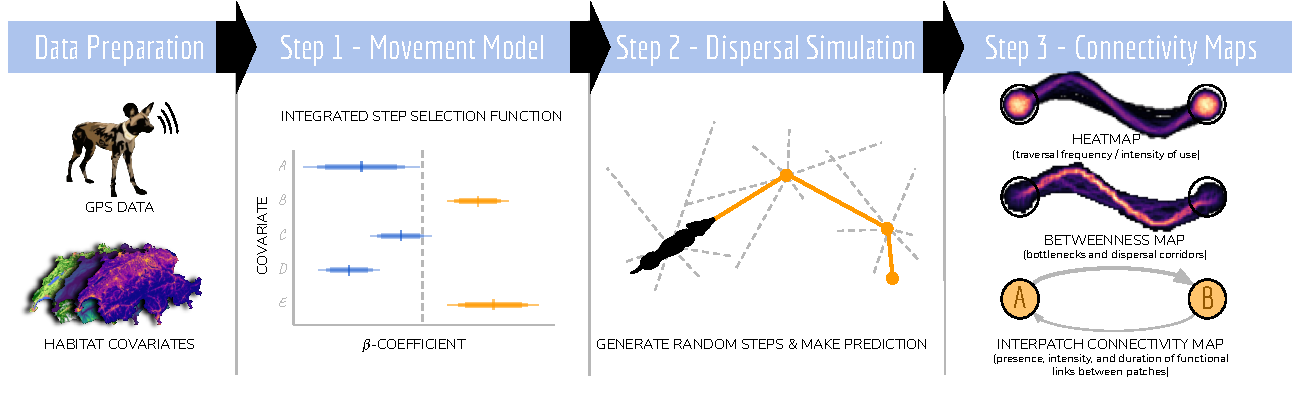
\includegraphics[width = \textwidth]{99_GraphicalAbstract.pdf}
    \caption{Flowchart of the simulation-based connectivity analysis. First, GPS
    data and habitat covariates have to be collected. The combined data is then
    analyzed in an integrated step selection model, which enables the
    parametrization of the focal species' habitat and movement kernels. The
    parametrized model is then treated as an individual-based movement model and
    used to simulate dispersal trajectories. Ultimately, simulated trajectories
    serve to produce a set of maps that are pertinent to landscape connectivity.
    This includes a heatmap, indicating the relative traversal frequency across
    the study area, a betweenness map, highlighting movement corridors and
    bottlenecks, and, finally, an inter-patch connectivity map, where the
    frequency of connections and their average duration can be depicted. Photos:
    Whom to cite? Vectronics or Photographers?}
    \label{GraphicalAbstract}
  \end{center}
\end{figure}

\section{Methods}
\subsection{Study Area (90\%)}
The study area was defined by a bounding box centered at -17\degree 13'9''S,
23\degree 56'4''E (\Cref{StudyArea}a) stretching over 1.3 Mio.
km\textsuperscript{2} and ecompassing the entire KAZA-TFCA (\Cref{StudyArea}b).
The KAZA-TFCA represents the world's largest transboundary conservation area and
comprises parts of Angola, Botswana, Namibia, Zimbabwe, and Zambia. It covers a
total of 520'000 km\textsuperscript{2} and hosts a diverse landscape, ranging
from savanna to grassland and from dry to moist woodland habitats. In its center
lies the Okavango Delta, a dominant hydrogeographical feature and the world's
largest flood-pulsing inland delta. The wet season within the KAZA-TFCA lasts
from November to March and is out of phase with the flood in the Okavango Delta,
which peaks between July and August \citep{McNutt.1996, Wolski.2017}. Although
large portions within the KAZA-TFCA are designated national parks or other
protected areas, considerable human influence remains due to roads, agricultural
sites and settlements and villages that are distributed across the KAZA-TFCA's
landscape.

\begin{figure}[htbp]
  \begin{center}
    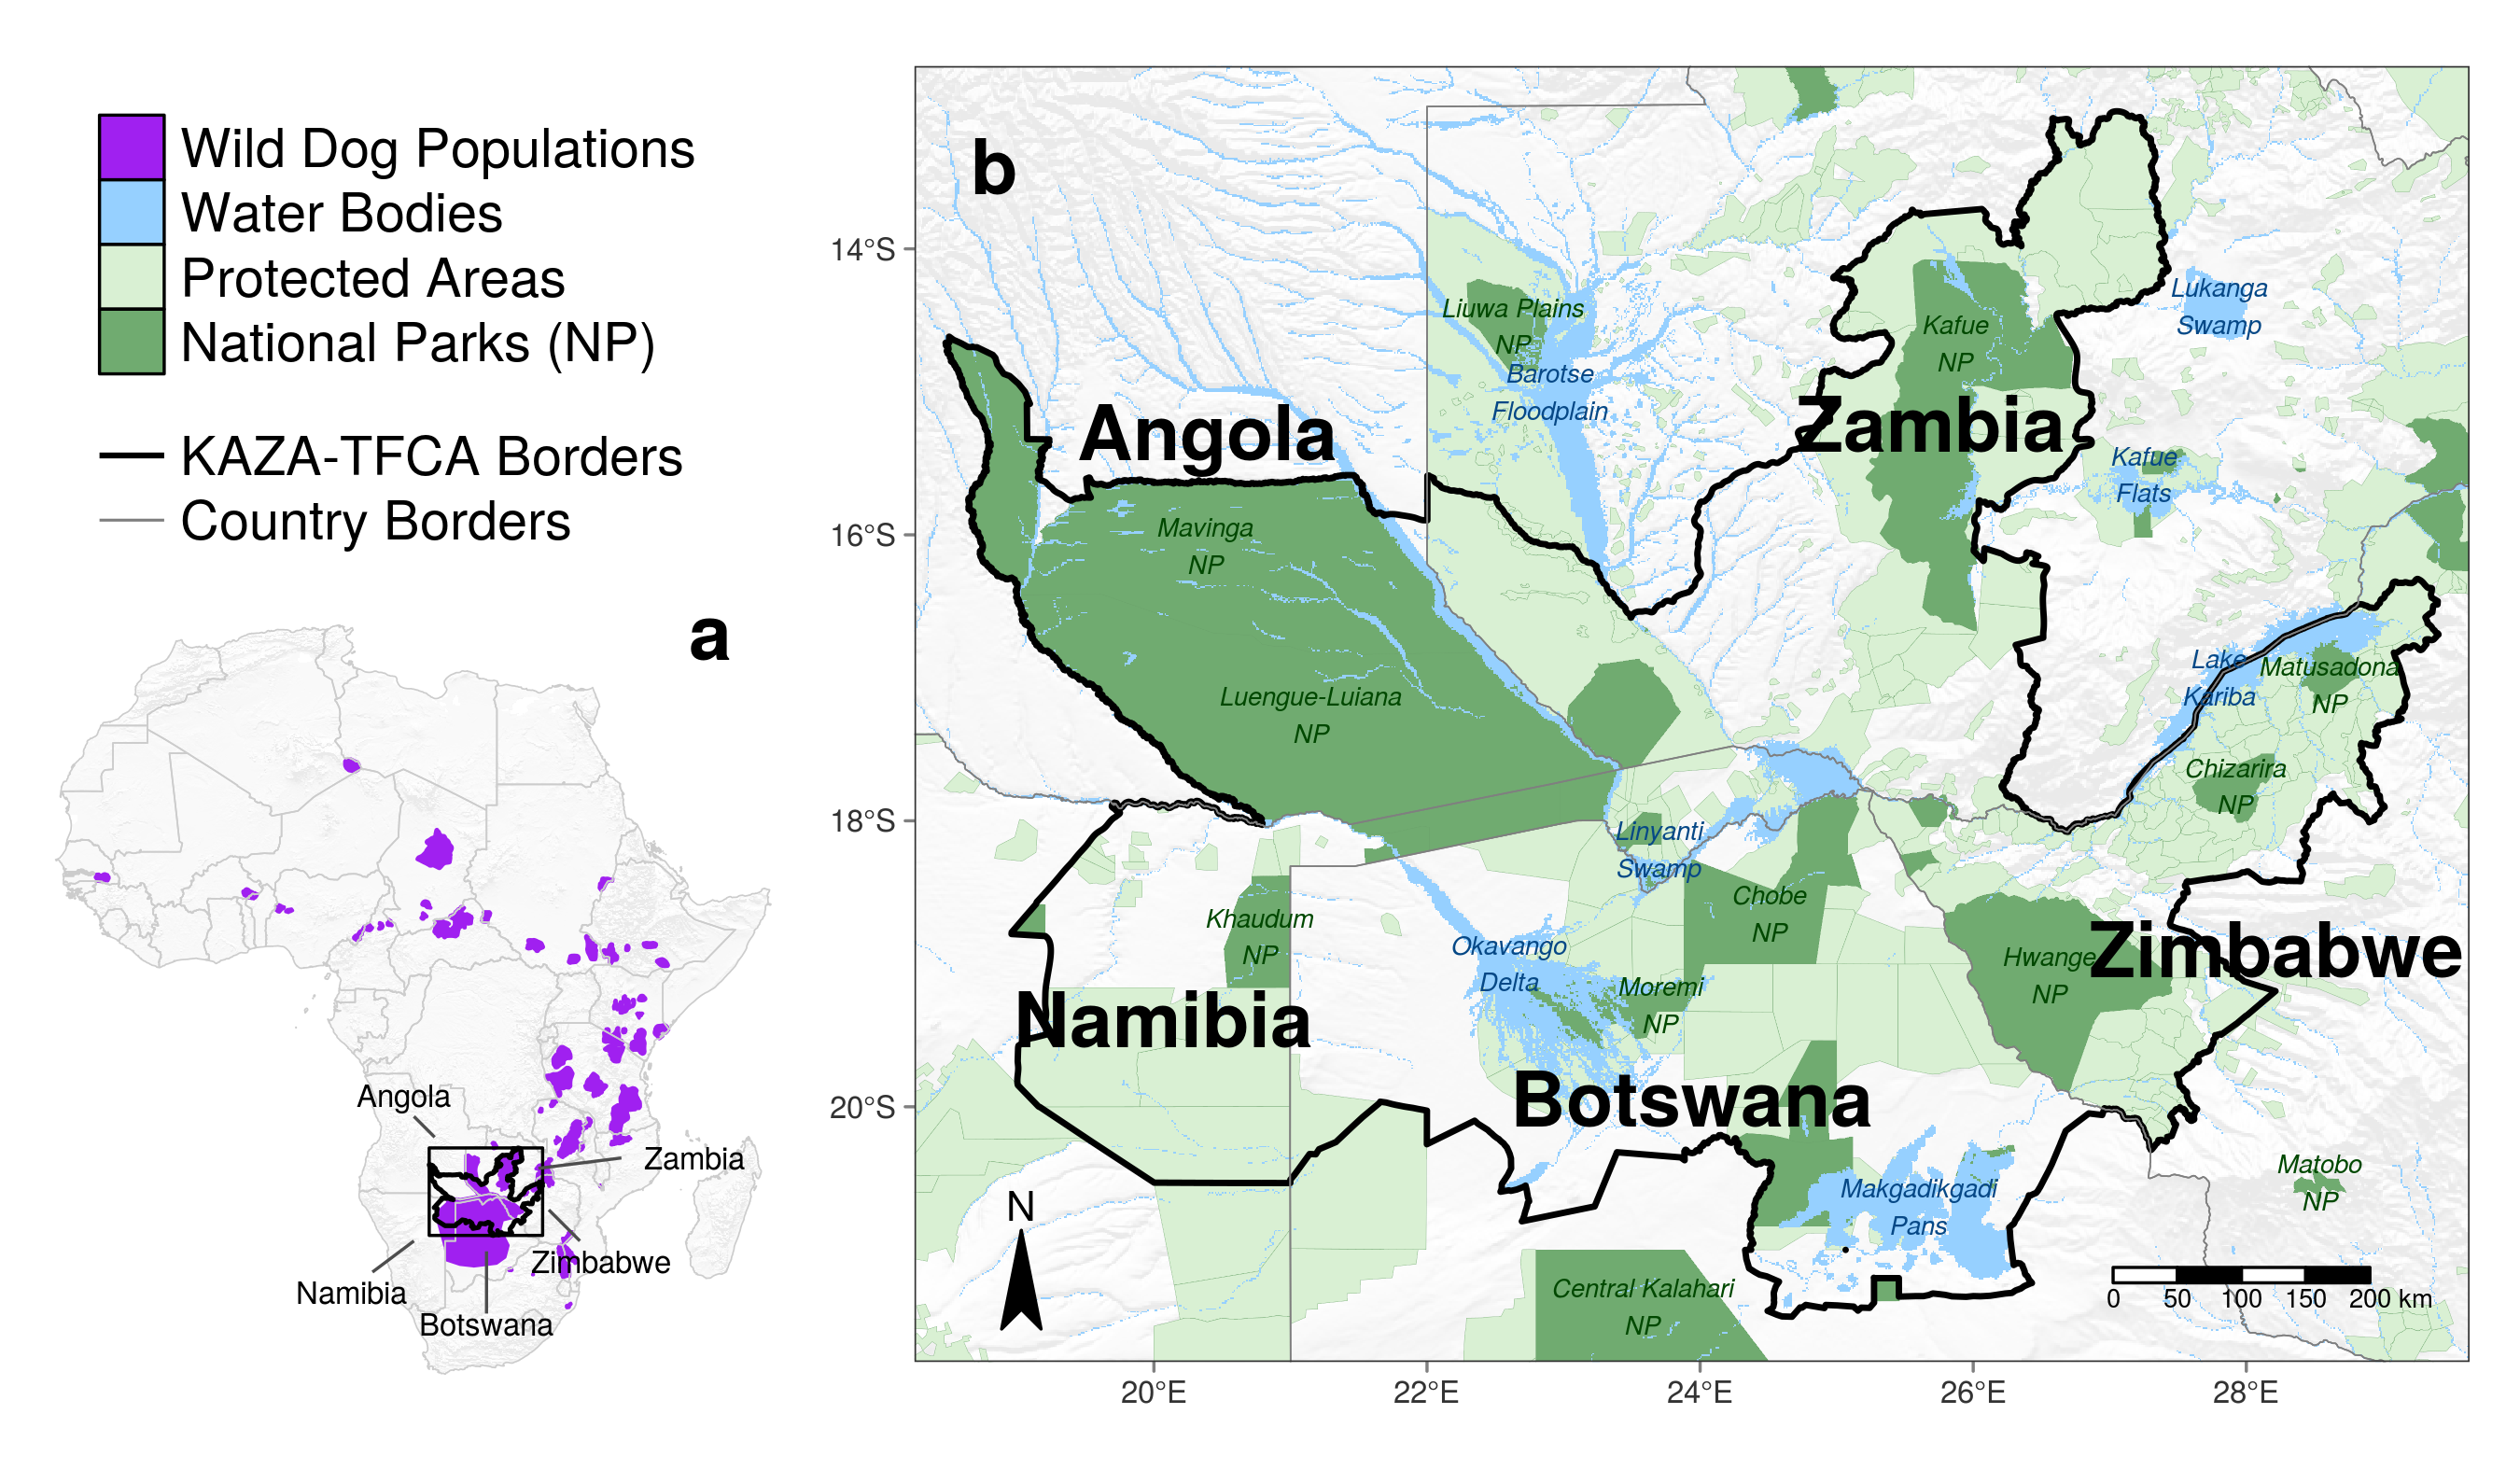
\includegraphics[width = \textwidth]{99_StudyArea.png}
    \caption{Illustration of the study area located in southern Africa. (a) The
    study area was confined by a bounding box spanning the entire KAZA-TFCA and
    encompassing parts of Angola, Namibia, Botswana, Zimbabwe, and Zambia. (b)
    The KAZA-TFCA represents the world's largest terrestrial conservation area
    and covers a total of 520'000 km\textsuperscript{2}. Its purpose is to
    re-establish connectivity between already-existing national parks (dark
    green) and other protected areas (light green). The dispersal data used in
    this study was collected on a free-ranging African wild dog population
    inhabiting the Moremi National Park in northern Botswana.}
    \label{StudyArea}
  \end{center}
\end{figure}

\subsection{GPS Relocation Data (90\%)}
Between 2011 and 2019, we collected GPS relocation data on dispersing wild dogs
from a free-ranging wild dog population inhabiting the Moremi National Park in
northern Botswana \citep{Cozzi.2020, Hofmann.2021}. We selected potential
dispersers based on age, pack size, number of same‐sex siblings within the pack,
and presence of unrelated opposite-sex individuals in the pack
\citep{McNutt.1996, Behr.2020}. We immobilized selected individuals using a
cocktail of Ketamine/Xylazine/Atropine \citep{Osofsky.1996, Cozzi.2020} that was
injected by dart, fired from a CO\textsubscript{2}-pressurized gun
(\textit{DAN-Inject, Denmark}). Immobilized individuals were fitted with
GPS/Satellite radio collars (\textit{Vertex Lite; Vectronic Aerospace GmbH,
Berlin}) that guaranteed automated drop-off through a decomposable piece of
cotton. Handling and collaring of all individuals was supervised by a
Botswana-registered wildlife veterinarian and all individuals quickly rejoined
their pack after immobilization.

16 collared individuals eventually dispersed, each in a separate same-sex
dispersal coalition (7 female and 9 male coalitions). During dispersal, collars
were programmed to record a GPS fix every 4 hours. Collected relocations were
regularly transmitted over the Iridium satellite system, which allowed remote
tracking of individuals, even if they left the main study area and crossed
international borders. Because behavior during dispersal is more pertinent for
assessing landscape connectivity \citep{Elliot.2014, Abrahms.2017}, we discarded
all data that was collected during residency and only retained GPS data recorded
during dispersal. In some instances, exact dispersal dates were known from field
observations. Where this was not the case, determined dispersal phases using the
net-squared displacement metric. Net squared displacement measures the squared
Euclidean distance of a GPS relocation to a reference point \citep{Borger.2012},
which in our case was set to the center of each individual's natal home range.
As such, dispersal was deemed to have started when an individual left its natal
home range and ended once individuals became sedentary again. As previous
research revealed similar behavior of females and males during dispersal
\citep{Woodroffe.2019, Cozzi.2020}, we did not distinguish between sexes. After
collection, we converted collected GPS coordinates (n = 4'169) to steps, where
each step represented the straight-line distance traveled by and individual
between two consecutive GPS relocations \citep{Turchin.1998}. To ensure a
regular sampling interval, we removed fixes that were not successfully collected
on the 4-hourly schedule (\( \pm \) 15 minutes).

\subsection{Covariates (90\%)}
We represented the physical landscape across the study area using a set of
habitat covariates that included water-cover, distance to water, woodland-cover,
and shrub/grassland-cover. Because water cover greatly changes within and
between years in the Okavango Delta, we applied a remote sensing algorithm and
generated frequently updated water cover layers and corresponding distance to
water layers (see \citealp{Wolski.2017} and Appendix A3 in
\citealp{Hofmann.2021}). Resulting water layers thus temporally aligned with our
dispersal events. We furthermore computed a proxy for human influence, rendering
anthropogenic pressures stemming from human-density, agricultural sites, and
roads. All spatial layers were coarsened or interpolated to a target resolution
of 250 m by 250 m. Further details on the sources and preparation of each
habitat covariate are given in \cite{Hofmann.2021}.

Besides habitat covariates, we computed movement metrics that we used as
movement covariates in our models. Movement metrics were calculated for each
step and included the step length (\textsf{sl}), its natural logarithm
(\textsf{log(sl)}), and the cosine of the relative turning angle
(\textsf{cos(ta)}) (for details see \citep{Avgar.2016, Fieberg.2020}). Because
wild dogs follow a diurnal activity pattern, we also coded a binary variable
(\textsf{LowActivity}) indicating whether a step was realized during periods of
low wild dog activity (17:00 to 09:00 local time) or high wild dog activity
(09:00 to 17:00 local time). Handling and manipulation of all data, as well as
all models and simulations were implemented with the statistical software {\tt
R}, version 3.6.6 \citep{R.2019}. Several helper functions were written in {\tt
C++} and imported into {\tt R} using the {\tt Rcpp} package
\citep{Eddelbuettel.2011, Eddelbuettel.2013}

\subsection{Movement Model (80\%)}
We used ISSFs to parametrize a mechanistic movement model for dispersing wild
dogs \citep{Avgar.2016}. To conduct ISSF analysis, we paired each realized step
with 24 random steps. An observed and its 24 random steps formed a stratum and
received a unique identifier. We generated random steps by sampling random
turning angles from a uniform distribution (\(-\pi, +\pi\)) and step lengths
from a gamma distirbution that was fitted to realized steps (scale = 6'308,
shape = 0.37). Along each step, we extracted and averaged spatial covariates
using the {\tt velox} package \citep{Hunziker.2017}. We also calculated the
movement metrics \textsf{sl}, \textsf{log(sl)}, and \textsf{cos(ta)} for each
observed and random step. To facilitate model convergence, we standardized all
continuous covariates to a mean of zero and a standard deviation of one. Since
correlation among covariates was low (\(|r| > 0.6\); \citealp{Latham.2011}), we
retained all of them for modeling.

To contrast realized steps (scored 1) and random steps (scored 0), we assumed
that animals assigned a selection score \(w(x)\) of the exponential form to each
step \citep{Fortin.2005}. The selection score \(w(x)\) of each step depended on
its associated covariates (\(x_1, x_2, ..., x_n\)) and on the animal's
preferences (i.e. relative selection strengths; \citealp{Avgar.2017}) towards
these covariates (\(\beta_1, \beta_2, ..., \beta_n\)):

\begin{equation}
\label{EQ1}
  w(x) = exp(\beta_1 x_1 + \beta_2 x_2 + ... + \beta_n x_n)
\end{equation}

The probability of a step being realized was then contingent on the step's
selection score, as well as on the selection scores of all other step in the
same stratum:

\begin{equation}
\label{EQ2}
  P(Y_{i} = 1 | Y_{1} + Y_{2} + ... + Y_{i} = 1) =
  \frac{w(x_{i})}{w(x_{1}) + w(x_{2}) + ... + w(x_{i})}
\end{equation}

To estimate the preferences of interest, we ran conditional logistic regression
analysis in the r-package {\tt glmmTMB}. To handle multiple individuals, we
applied the mixed effects technnique developed by \citep{Muff.2020}, which
allows to effectively model random slopes. Thus, we treated animal IDs as random
effect and modeled random slopes for each covariate. We fixed the random
intercept variance at an arbitrary high value of 10\textsuperscript{6} to make
use of the  ``poission''-trick \citep{Muff.2020}.

The formula for the movement model was based on the habitat selection model for
dispersing wild dogs presented in \cite{Hofmann.2021}. In the original model, no
interactions between habitat covariates (\textsf{Water,
DistanceToWater\textsuperscript{0.5}, Woodland, Shrubs/Grassland, Human
Influence}) and movement covariates (\textsf{sl, log(sl), cos(ta)}) were
considered. Here, we slightly expanded this base model and proposed interactions
between all movement and habitat covariates. More specifically, we started with
the base model and incrementally increased model complexity by adding all
possible two-way interactions between habitat covariates and movement
covariates. For instance, for the covariate \textsf{Water}, we proposed the
interactions \textsf{Water:log(sl)}, \textsf{Water:log(sl)}, and
\textsf{Water:cos(ta)}. Besides those combinations, we also proposed the
interactions \textsf{sl:cos(ta)} and \textsf{log(sl):cos(ta)} to account for a
correlation between turning angles and step lengths, as well as the interactions
\textsf{sl:LowActivity} and \textsf{log(sl):LowActivity} to account for the fact
that step lengths may differ due to wild dogs' diurnal activity pattern. To
compare competing models and assess the most parsimonious movement model, we ran
stepwise forward model selection based on Akaike's Information Criterion (AIC,
\citealp{Burnham.2002}).

We validated the predictive power of the most parsimonious movement model using
k-fold cross-validation for case-control studies as suggested by
\cite{Fortin.2009}. For this, we randomly assigned 80\% of the strata to a
training set and the remaining 20\% to a testing set. Using the training data we
parametrized a movement model based on which we predicted selection scores
\(w(x)\) for all steps in the test data. Within each stratum, we then assigned
ranks 1-25 to each step based on predicted selection scores, where rank 1 was
given to the step with the highest score \(w(x)\). Across all strata we
determined the realized step's rank and we calculated rank frequencies of
realized steps across all strata. Finally, we computed Spearman's rank
correlation between ranks and associated frequencies \(r_{s, realized}\). We
replicated the entire procedure 100 times and computed the mean correlation
coefficient (\(\bar{r}_{s, realized}\)), as well as its 95\% confidence interval
across all replicates. For comparison, we repeated the same procedure 100 times
assuming random preferences, which we implemented by discarding the realized
step from all strata and identifying the rank of a random step in each stratum.
Again, we calculated Spearman's rank correlation coefficient (\(r_{s,
random}\)), its mean across repetitions (\(\bar{r}_{s, random}\)), and its 95\%
confidence interval. This validation ultimately proofs a significant prediction
in case the confidence intervals of \(\bar{r}_{s, realized}\) and \(\bar{r}_{s,
random}\) do not overlap.

\subsection{Dispersal Simulation (80\%)}
We used the most parsimonious movement model to simulate 80'000 virtual
dispersers moving across the KAZA-TFCA. The simulation resembled an inverted
ISSF and was set up as follows. (1) We defined a random source point and assumed
a random initial orientation of the animal. (2) Departing from the source point,
we generated 25 random steps by sampling turning angles from a uniform
distribution (\(-\pi, +\pi\)) and step lengths from our fitted gamma
distribution. Similar to the input data, each random step represented the
straight line movement within 4 hours. To prevent unreasonably large steps, we
capped sampled step lengths to a maximum of 35 km, which corresponded to the
farthest distance ever traveled within 4 hours by one of our dispersers. (3)
Along each random step, we extracted and averaged habitat covariates and we
calculated movement covariates. To ensure compatible scales, we standardized
extracted values using the same parameters applied to our input data. (4) We
applied the parameterized movement model to predict the selection score
\(w(x)\), which we translated into probabilities using \Cref{EQ2}. (5) We
sampled one of the random steps based on predicted probabilities and determined
the animal's new position. We repeated steps (2) to (5) until 2'000 steps were
realized, implying a total 160 Mio. simulated steps.

To minimize the influence of edge effects and to deal with random steps leaving
the study area, we followed \citep{Koen.2010} and artificially expanded all
covariate layers by adding a 100 km wide buffer zone. Within the buffer zone, we
randomized covariate values by resampling values from the original covariate
layers. Through this buffer zone, simulated dispersers were able to leave and
re-enter the main study area. In cases where proposed random steps transgressed
the border of this buffer zone, we resampled transgressing steps until they
fully lied within the buffer, thereby forcing simulated individuals to ``bounce
off'' from such invisible borders.

\subsection{Source Points (90\%)}
We released 80'000 virtual dispersers from 80'000 unique source points
distributed across the study area. 50'000 virtual dispersers were released from
randomly selected source points within contiguous protected areas larger \(>\)
700 km\textsuperscript{2} (\Cref{SourcePoints}a), which conforms to average home
range requirements of resident wild dogs \citep{Pomilia.2015} and allowed us to
remove patches too small to host viable populations. By distributing source
points randomly, the number of source points per km\textsuperscript{2} was
approximately equal within protected areas. To render potential immigrants into
the study system, we released another 30'000 dispersers at random locations
inside the 100 km wide buffer zone surrounding the main study area
(\Cref{SourcePoints}b).

\begin{figure}[htbp]
  \begin{center}
    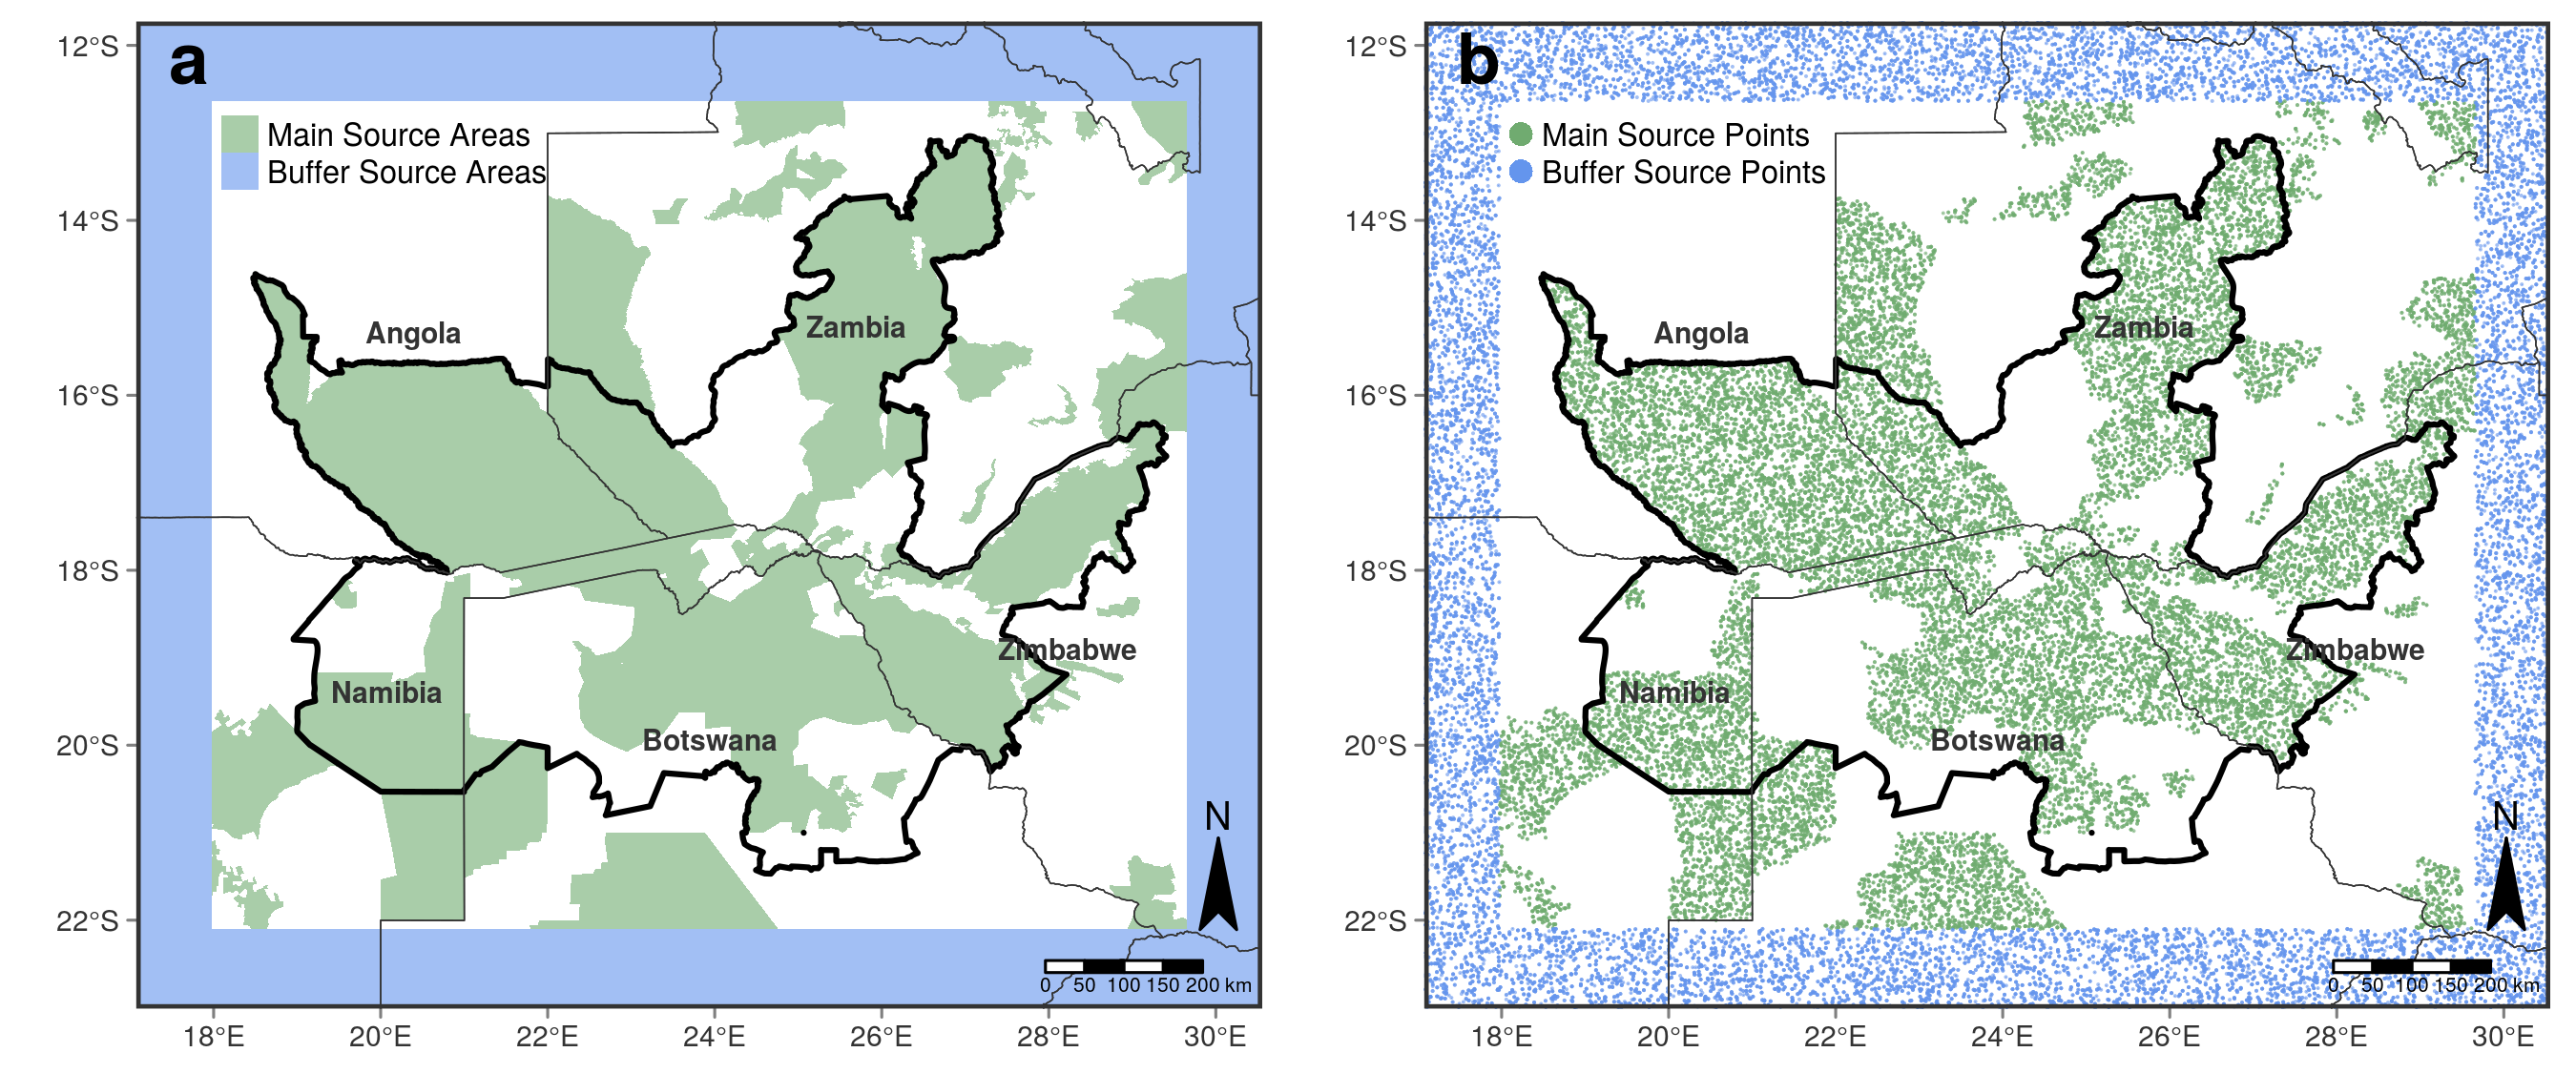
\includegraphics[width = \textwidth]{99_SourceAreas.png}
    \caption{(a) Different source areas from which we released virtual
    dispersers. We only considered contiguous protected areas (national parks,
    game reserves, and forest reserves) that were larger than 700
    km\textsuperscript{2} (green). This area corresponds to the average home
    range requirement for viable wild dog populations \citep{Pomilia.2015}. To
    render potential immigrants into the study system, we also initiated
    dispersers within a buffer zone (blue) surrounding the main study area. (b)
    Source points from which dipsersers were released. 50'000 dispersers were
    released from the main study area (green dots) and another 30'000 dispersers
    within the virtual buffer (blue dots).}
    \label{SourcePoints}
  \end{center}
\end{figure}

\subsection{Heatmap (100\%)}
To identify dispersal hotspots across our study area, we created a heatmap
indicating the absolute frequency at which each raster-cell in the study area
was visited by virtual dispersers. For this, we rasterized all simulated
trajectories and tallied them into a single map. If the same trajectory crossed
a raster-cell twice, it was only counted once. This way, we mitigated potential
biases resulting from trapped individuals that were moving in circles. To
achieve high performance rasterization, we used the R-package {\tt terra}
\citep{Hijmans.2020}.

\subsection{Betweenness (80\%)}
To pinpoint areas of exceptional relevance for connecting remote regions in our
study area, we converted simulated trajectories into a network and calculated
betweenness scores. For this, we overlaid the study area (including the buffer)
with a regular raster resolved at 5 x 5 km. The centerpoint of each raster-cell
acted as node in the final network and we used the simulated trajectories to
determine all transitions occurring from one raster-cell to another, as well as
the frequency at which those transitions occurred. This resulted in an edge-list
that we translated into a weighted network using the r-package {\tt igraph}
\citep{Gabor.2006}. Because {\tt igraph} handles edge weights (\(\omega\)) as
costs, we inverted the traversal frequency in each cell by applying \(\omega =
\frac{\sum_i^n{Traversal Frequency_i}/n}{Traversal Frequency_i}\). Finally, we
used the weighted network to calculate the betweenness score of each
raster-cell. Betweenness measures how often a specific raster-cell lies on a
shortest path between two other raster-cells and is therefore a useful metric to
detect movement corridors \citep{BastilleRousseau.2018}.

\subsection{Inter-Patch Connectivity (80\%)}
To exemplify how simulations can be used to provide a network view on
connectivity, we assessed inter-patch connectivity between national parks
located in our study area. The decision to focus on national parks was purely
out of simplicity and does not imply that connections between other regions are
impossible. In fact, the same logic could easily be expanded to include other
protected areas as well. To quantify inter-patch connectivity, we computed the
relative frequency at which dispersers originating from one national park
successfully moved into another national park. Successful movement was said to
be achieved if the individuals' trajectory ever intersected with the
corresponding national park. We also recorded the step-number of the first step
that ever intersected with the national park's polygon. This allowed us to
determine \textit{if} and \textit{how often} dispersers moved between certain
national parks, as well as to estimate \textit{how long} dispersers had to move
to realize those connections.

\section{Results}
\subsection{Movement Model (60\%)}
Compared to the base model reported in \citep{Hofmann.2021}, our most
parsimonious movement model contained several additional interactions between
habitat covariates and movement covariates (\Cref{MovementModel} and
\Cref{MovementModelNumbers}). Although multiple models received an AIC weight
above zero (Table 1 in Appendix S1), we only considered results from the most
parsimonious model. Since all models with positive AIC weight contained similar
covariates (Table S1), this decision only marginally influenced subsequent
analyses. Plots that aid with the interpretation of the final model are provided
in Appendix S2.

When looking at the habitat kernel (and holding constant the movement kernel),
we find that dispersing wild dogs avoid water but prefer its proximity.
Dispersers also avoid woodlands, yet prefer shrublands or grasslands. Finally,
dispersers avoid moving through landscapes that are influenced by humans. These
results align with our previous findings reported in \cite{Hofmann.2021}.

Results from the movement kernel indicate several significant estimates.
However, except for the interaction \textsf{sl:LowActivity}, effect sizes are
relatively small, indicating that our proposal distributions for step lengths
and turning angles were only marginally biased by habitat selection. For
instance, the positive and significant estimate for \textsf{cos(ta)} indicates
that realized turning angles were slightly more directional than the turning
angles proposed by our uniform distribution. This shows that realized steps in
reality followed a von Mises Distribution with positive concentration parameter.
On the other hand, the significant and negative interaction for
\textsf{sl:LowActivity} reveals that wild dogs realized shorter steps during low
wild dog activity compared to the steps suggested by our gamma distribution.

When looking at the interactions between the movement and habitat kernel, we
observe several significant interactions, highlighting that movement behavior
differs depending on habitat conditions. For example, there's ample evidence
that the propensity to realize a log step in areas covered by water is
substantially smaller compared to the propensity of realizing a small step.
Similarly, long steps are less likely to be realized in areas covered by trees,
compared to more open regions. Conversely, it appears that steps tend to longer
be in the vicinity to water, even though the size of this effect is negligible.
Finally, it seems that dispersers move more tortuous in areas influenced by
humans, but more directional when far from water.

The k-fold cross-validation procedure reveals that our model substantially
outperforms a random guess (\Cref{MovementModel}b). Confidence intervals of
\(\bar{r}_{s, realized}\) and \(\bar{r}_{s, random}\) do not overlap and
therefore proof a reliable prediction. Furthermore, the significant correlation
between ranks and corresponding frequencies for realized steps indicates a good
fit between predictions and observations (\Cref{MovementModel}b). In comparison
to the base model (\(\bar{r}_{s, realized} = -0.55\); \citealp{Hofmann.2021}),
the inclusion of interactions between movement and habitat covariates slightly
improved model performance.

\begin{figure}
  \begin{center}
    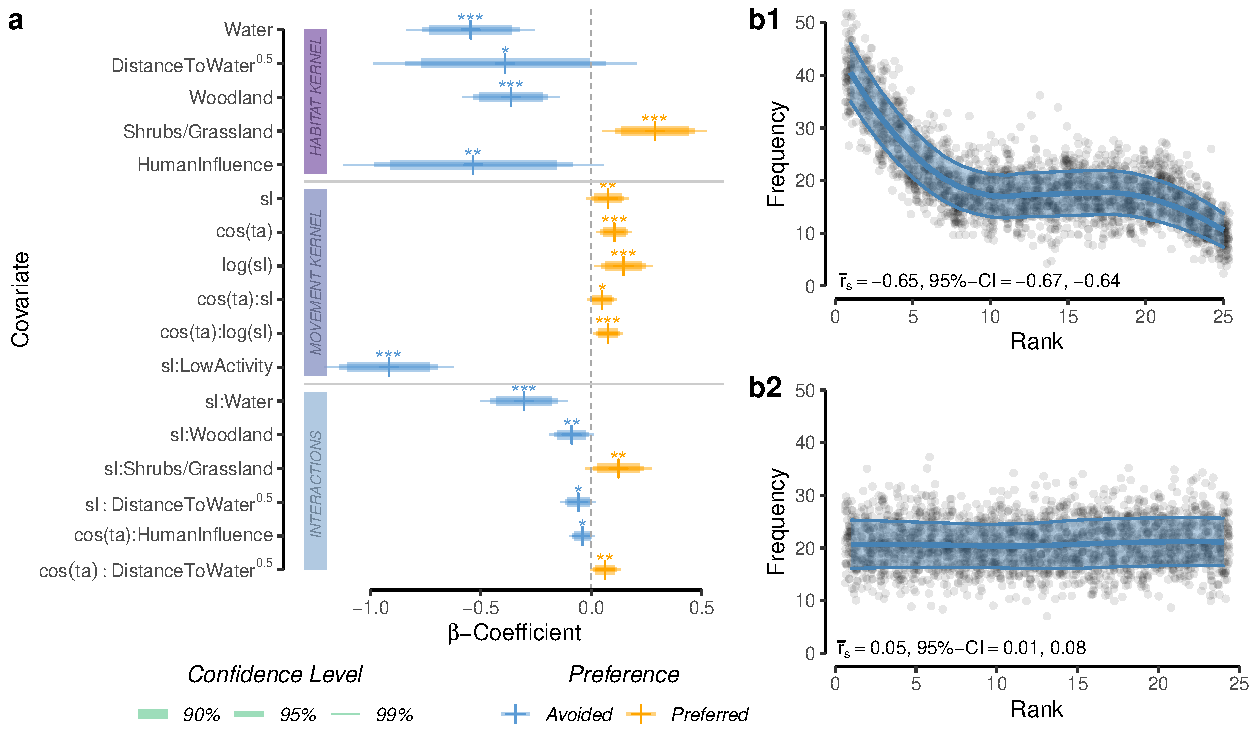
\includegraphics[width=\textwidth]{99_MovementModel}
    \caption{(a) Most parsimonious movement model for dispersing wild dogs. The
    model includes a habitat kernel, a movement kernel, as well as their
    interactions. The orange and blue line segments delineate the 90\%, 95\%,
    and 99\% Confidence-Intervals around the respective \(\beta\) coefficients.
    Significance codes: * \(p < 0.10\), ** \(p < 0.05\), *** \(p < 0.01\). (b)
    Results from the k-fold cross validation procedure. The upper plot shows
    rank frequencies of predicted realized scores according to model predictions
    with known preferences, whereas the lower plot shows rank frequencies when
    assuming random preferences. The blue ribbon shows the prediction interval
    around a loess smoothing regression that we fitted to ease the
    interpretation of the plots.}
    \label{MovementModel}
  \end{center}
\end{figure}

\begin{table}
  \begin{center}
  \caption{Most parsimonious movement model for dispersing wild dogs. The model
  consists of a movement kernel, a habitat kernel, and their interactions. The
  movement kernel describes preferences with regards to movement behavior,
  whereas the habitat kernel describes preferences with respect to habitat
  conditions. Interactions between the two kernels indicate that movement
  preferences are contingent on habitat conditions. Note that all covariates
  were standardized to a mean of zero and standard deviation of 1. Plots to aid
  with the interpretation of this model are given in Appendix S2.}
  \label{MovementModelNumbers}
  \resizebox{\textwidth}{!} {
    \begin{threeparttable}
      \begin{tabular}{llrrrc}
        \toprule
        Kernel & Covariate & Coefficient & SE & p-value & Sign. \\
        \midrule
        \multirow{5}{*}{Habitat Kernel}
         & Water & -0.546 & 0.112 & \(<\) 0.001 & *** \\
         & DistanceToWater \textsuperscript{0.5} & -0.390 & 0.231 & 0.092 & * \\
         & Woodland & -0.364 & 0.086 & \(<\) 0.001 & *** \\
         & Shrubs/Grassland & 0.288 & 0.092 & 0.002 & *** \\
         & HumanInfluence & -0.535 & 0.229 & 0.019 & ** \\
        \hdashline
        \multirow{6}{*}{Movement Kernel}
         & sl & 0.075 & 0.037 & 0.042 & ** \\
         & cos(ta) & 0.105 & 0.031 & 0.001 & *** \\
         & log(sl) & 0.146 & 0.051 & 0.004 & *** \\
         & cos(ta) : sl & 0.049 & 0.026 & 0.064 & * \\
         & cos(ta) : log(sl) & 0.076 & 0.026 & 0.003 & *** \\
         & sl : LowActivity & -0.917 & 0.113 & \(<\) 0.001 & *** \\
        \hdashline
        \multirow{5}{*}{Interaction}
         & sl : Water & -0.305 & 0.076 & \(<\) 0.001 & *** \\
         & sl : Woodland & -0.089 & 0.039 & 0.023 & ** \\
         & sl : Shrubs/Grassland & 0.124 & 0.058 & 0.032 & ** \\
         & sl : DistanceToWater \textsuperscript{0.5} & -0.058 & 0.031 & 0.056 & * \\
         & cos(ta) : HumanInfluence & -0.040 & 0.022 & 0.070 & * \\
         & cos(ta) : DistanceToWater \textsuperscript{0.5} & 0.063 & 0.026 & 0.017 & ** \\
         \bottomrule
      \end{tabular}
       \begin{tablenotes}
         \item \textit{Significance codes: * \(p < 0.10\) \quad ** \(p < 0.05\)
         \quad *** \(p < 0.01\)}
       \end{tablenotes}
    \end{threeparttable}
    }
  \end{center}
\end{table}

\subsection{Dispersal Simulation (80\%)}
On a machine with an octacore AMD Ryzen 7 2700X processor (8 x 3.6 GHz) and 64
GB of RAM, a single batch of 1'000 simulated dispersers took roughly 90 minutes
to compute (\(\mu = 88.90\), \(\sigma = 1.87\)) and the simulation of all 80'000
dispersers terminated after 120 hours, i.e. five days. Comparable computations
will be substantially faster for smaller study areas or lower resolution
covariates, as the covariate extraction from large rasters was computationally
the most expensive task.

On average, step lengths realized by the simulated dispersers (\(\mu_{sl} =
2'093\) m, \(\sigma_{sl} = 3'067\)) were slightly shorter than those by observed
dispersers (\(\mu_{sl} = 2'326\) m, \(\sigma_{sl} = 3'323\)) and simulated
dispersers moved marginally less directional (\(\mu_{cos(ta)} = 0.057\),
\(\sigma_{cos(ta)} = 0.071\)) compared to observed dispersers (\(\mu_{cos(ta)} =
0.078\), \(\sigma_{cos(ta)} = 0.072\)). These differences in step lengths and
turning angles can be attributed to minor disparities between habitat conditions
at the area within which we collected training data and habitat conditions
within the entire study area. Out of the 50'000 dispersers initiated in
protected areas, only 4.5\% eventually hit a map boundary, suggesting that
biases due to boundary effects should be limited. In contrast, 78\% of the
30'000 dispersers originating from the buffer zone eventually hit a map
boundary.

\subsection{Heatmap (80\%)}
\Cref{Heatmap} depicts the heatmap of all 80'000 simulated trajectories rendered
after 2'000 steps. The map highlights that large portions of land beyond the
borders of the KAZA-TFCA are only infrequently visited by dispersers (dark blue
areas), whereas within the KAZA-TFCA several extensive regions are regularly
visited (bright yellow and red areas). Most notably, the region in northern
Botswana south of the Linyanti swamp stands out as highly frequented dispersal
hub. Still, the presence of several massive water bodies, such as the Okavango
Delta, the Makgadikgadi Pan, and the Linyanti swamp, results in considerable
dispersal barriers that limit realized connectivity within the KAZA-TFCA.
Similarly, dispersal appears to be very limited in Zambia's and Zimbabwe's part
of the KAZA-TFCA, where only few areas are regularly traversed by dispersers.
This which can largely be attributed to the strong high human influences in
these regions. Outside the KAZA-TFCA, the most heavily trafficked regions
include the areas of the Central Kalahari National Park in Botswana, the area
south-west of the Khaudum National Park in Namibia, and the area around the
Liuwa Plains National Park in Zambia.

\begin{figure}
  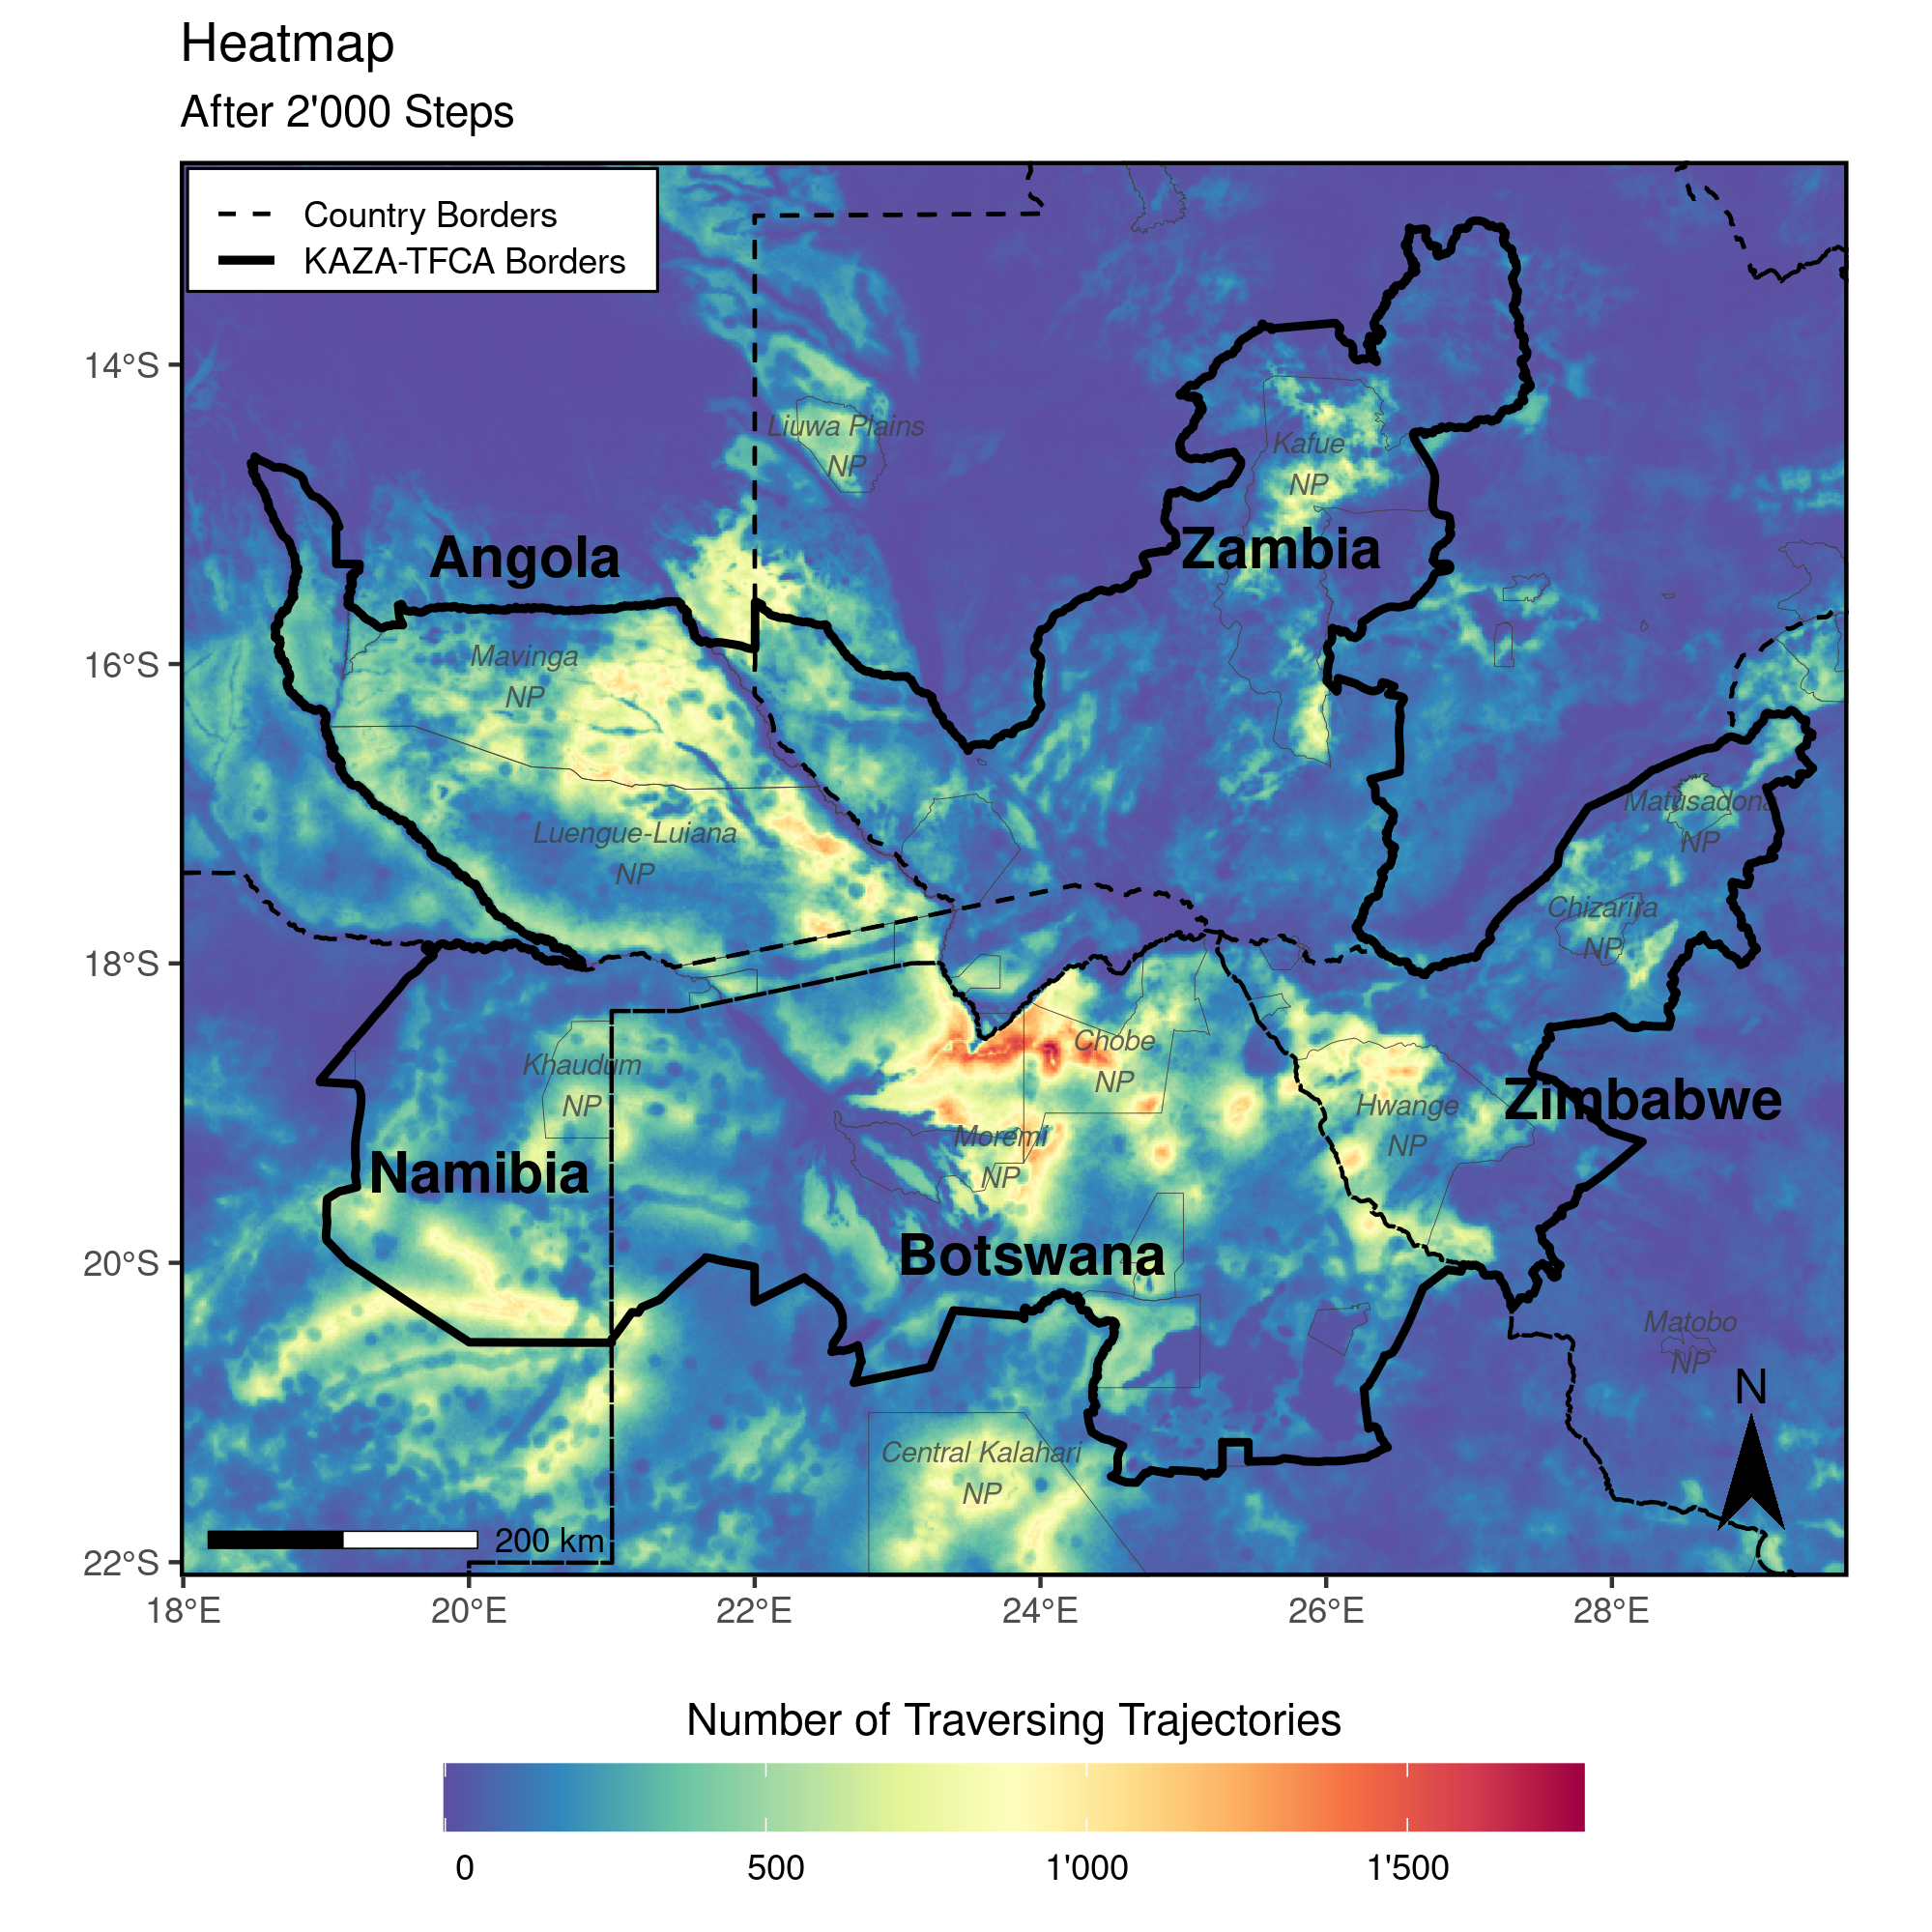
\includegraphics[width=\textwidth]{99_Heatmap.png}
  \caption{Heatmap showing traversal frequencies of 80'000 simulated dispersers
  moving 2'000 steps across the KAZA-TFCA. Simulations were based on an
  integrated step selection model that we fit to the movement data of dispersing
  African wild dogs. To generate the heatmap, we rasterized and tallied all
  simulated trajectories. Consequently, the map highlights areas that are
  frequently traversed by virtual dispersers. Further heatmaps showing the
  traversal frequency after different numbers of steps are provided in Appendix
  S3.}
  \label{Heatmap}
\end{figure}

\subsection{Betweenness (80\%)}
Betweenness scores of each raster-cell the study area are presented in
\Cref{Betweenness} and reveals a set of discrete dispersal corridors. As can be
seen, the dispersal hotspot in northern Botswana reported above is crossed by
a corridor that receives a relativley high betweenness score. This implies that
the region is particularly crucial for connecting other regions in the study
system and hence represents a proper hub in the  ``network'' . Towards east, the
corridor runs through the Chobe National Park into the Hwange national park,
where it branches out and further extends into the distant Matusadona National
Park in Zimbabwe. Northwest of the Linyanty ecosystem, the same corridor expands
into Angola, where it splits and finally traverses over a long stretch of
unprotected area into the Kafue National Park in Zambia. Several additional
corridors with slightly lower betweenness scores exist, yet most of them run
within the boundaries of the KAZA-TFCA. In general, only few corridors directly
link the peripheral regions of the KAZA-TFCA. For instance, there are only few
corridors between the Matusadona National Park in Zimbabwe and the Kafue
National Park in Zimbabwe. Similarly, there are no direct links between the
Zimbabwean and Angolan ``spikes'' of the KAZA-TFCA.

\begin{figure}
  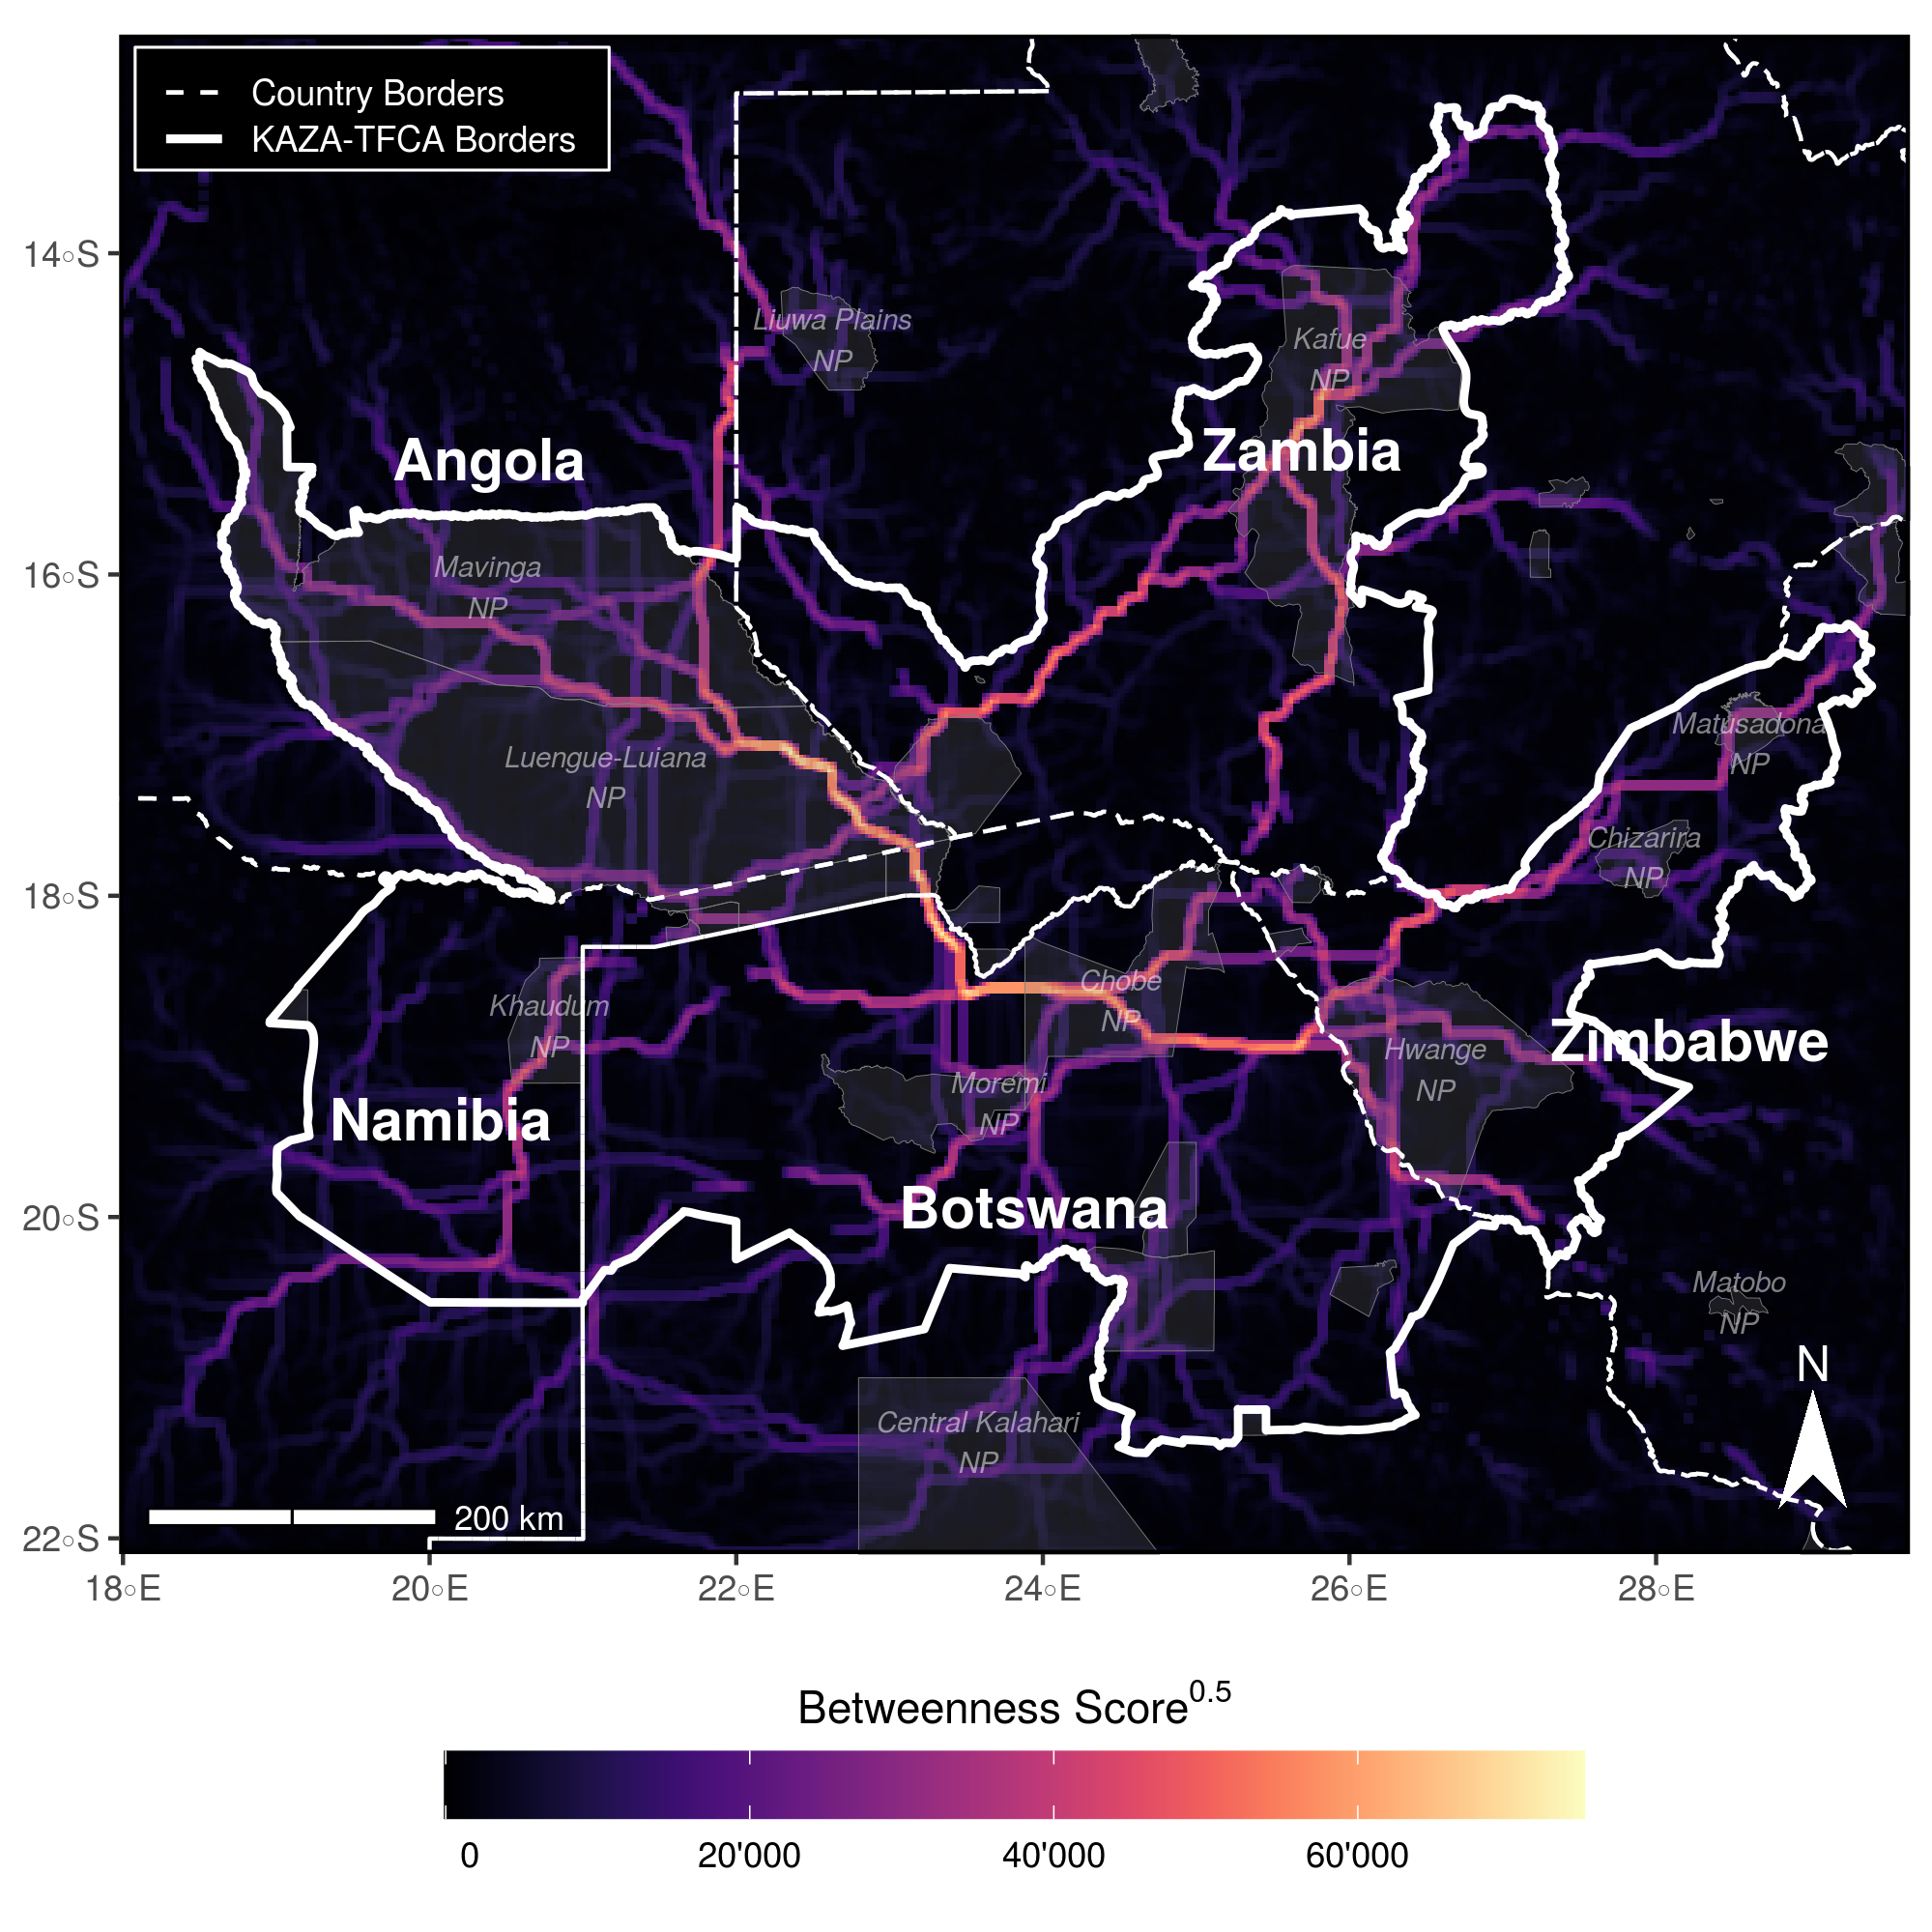
\includegraphics[width=\textwidth]{99_Betweenness.png}
  \caption{Betweenness scores of each raster cell in a raster with 5 x 5 km
  resolution. Betweenness scores were determined based on simulated dispersal
  events. A high betweenness score highlights cells that are exceptionally
  relevant in connecting different regions in the study area. That is, the
  higher the betweenness score, the more often a pixel lies on a shortest path
  between adjacent areas. In this sense the metric can be used to pinpoint
  discrete movement corridors. Note that we square-rooted betweenness scores to
  improve visibility of corrdiors with low scores.}
  \label{Betweenness}
\end{figure}

\subsection{Interpatch Connectivity (50\%)}
Results from the analysis of interpatch connectivity are given in
\Cref{AreasReached}. It is worth pointing out that the figure is only intended
as an example; for clarity we limited the network on national parks, albeit
plenty of links to other protected areas exist. The map shows all realized links
by simulated dispersers between national parks and indicates the average
duration a disperser had to move to realize those links. For instance, 6.8 \% of
the simulated dispersers originating from the Moremi National Park successfully
reached the Chobe National Park and 4.2 \% the Hwange National Park in Zimbabwe.
On average, dispersers moved for 623 steps before arriving at Chobe (SD = 520)
and for 1'413 steps before arriving at Hwange (SD = 371). While the map only
depicts connections between national parks, this does not imply that no
connections to other protected areas exist and is the result of our simplifying
assumptions above. Interestingly, while we identified a potential dispersal
corridor between Angola's NPs and the Kafue NP in Zambia, \Cref{AreasReached}
suggests that this link is only rarely realized and requires very long dispersal
events. In contrast, we find that dispersal between the Moremi NP and Chobe NP
are relatively frequent and require fewer steps, which can be expected given
that the areas are located close to each other.

\begin{figure}
  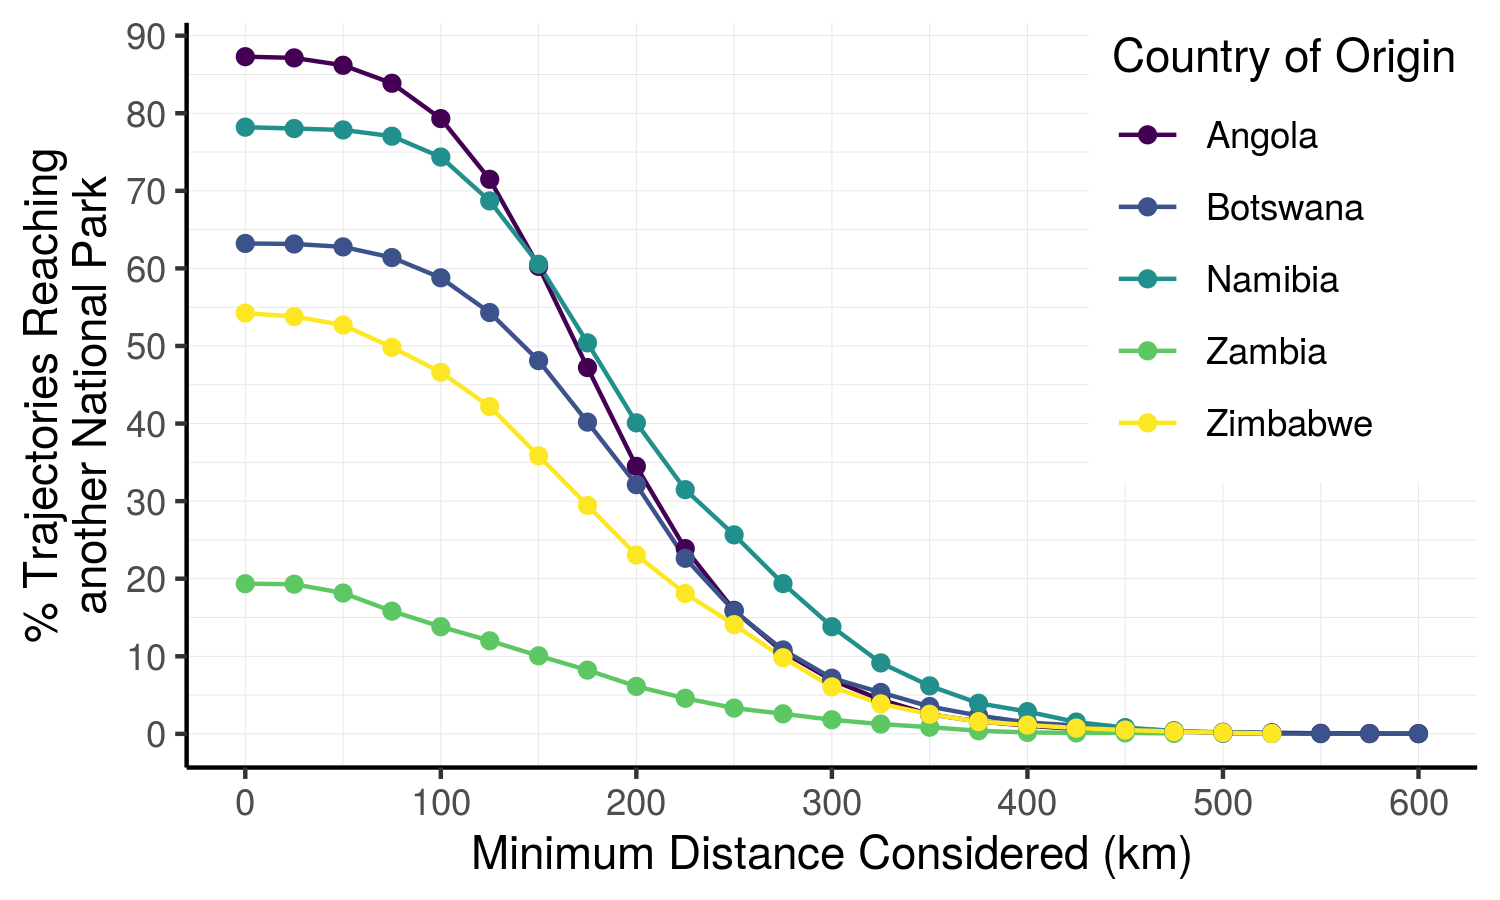
\includegraphics[width=\textwidth]{99_AreasReached.png}
  \caption{Network on simulated dispersal trajectories highlighting connections
  between national parks (dark green). Yellow bubbles represent the center of
  the different national parks and are sized in relation to the number of
  simulated dispersers originating from each park. Black dots represent national
  parks that were smaller than 700 km\textsuperscript{2} and therefore did not
  serve as source areas. Arrows between national parks illustrate between which
  national parks the simulated dispersers successfully moved and the color of
  each arrow shows the average number of steps (4-hourly movements) that were
  necessary to realize those connections. Additionally, the line thickness
  indicates the relative number of dispersers originating from a national park
  that realized those connections. Note that a similar network view could be
  adopted to investigate connectivity between other protected areas need not to
  be restricted to national parks.}
  \label{AreasReached}
\end{figure}

\section{Discussion}
\subsection{Short Summary (90\%)}
To this end, we used integrated step selection functions to analyse data of
dispersing wild dogs and parametrize a fully mechanistic movement model
describing how dispersers move through the available landscape. We employed the
parametrized model to simulate 80'000 dispersing wild dogs, moving across the
extent of the KAZA-TFCA, the world's largest transboundary conservation area.
Based on simulated dispersal trajectories, we prepared a set of complementary
maps, all geared towards a better understanding of dispersal and landscape
connectivity. The set of maps included a heatmap, revealing frequently traversed
areas, a betweenness-map, delineating critical dispersal corridors connecting
different regions, and a map of inter-patch connectivity, indicating presence or
absence of functional links between national parks, as well as the average
dispersal duration required realize those links. With this, we showcase that
integrated step selection analysis holds the potential to serve as simple, yet
powerful mechanistic movement model to simulate animal movement and assess
landscape connectivity. Importantly, such an individual-based approach overcomes
several shortcomings of traditional connectivity models, such as least-cost
analyses and circuit theory. Nevertheless, we support the idea that simulations
only serve as a complement, and not as substitute to more traditional
connectivity modeling techniques.

\subsection{Movement Model (50 \%)}
Our most parsimonious movement model comprised of a habitat kernel and a
movement kernel that describe in detail how dispersers move through the
available landscape. Parameter estimates revealed that dispersing wild dogs
avoid water, prefer proximity to water, avoid woodland, prefer shrubs/grassland,
and avoid areas dominated by humans. This is in line with an earlier dispersal
model, were we primarily investigated the habitat kernel \cite{Hofmann.2021},
and suggests that the introduction of additional covariates only marginally
impacted qualitative results. Even though corresponding effect sizes were
moderate, the model suggested that movement behavior of dispersers differs
depending on habitat characteristics. For instance, step lengths appear to be
shorter (i.e. animals move slower) in areas covered by water in comparison to
steps realized on dryland. We found similar interactions between movement
covariates and other habitat covariates, highlighting how a simple ISSF can be
employed to model relatively complex dispersal patterns. Correspondingly, the
ISSF framework allowed us to generically model resting behavior by including a
binary variable, signalling that dispersers moved were substantially slower
between 17:00 and 09:00 o'clock compared to the rest of the day.

While this (shorter steps on water) could be caused by a bias in our data,
where the straight line distance between two GPS relocations erroneously
suggests movement through water, where in reality the animal circumvented
water-bodies, we hypothesize that this slow-down is caused by dispersers that
move through the KAZA-TFCA's floodlands and get trapped by the flood. In fact,
we repeatedly observed individuals venturing across the Okavango Delta,
suddenly getting surrounded by the advancing flood. Until the flood retracts,
these individuals often remain on distinct ``islands'' on which movement is
restricted to rather small steps. This also aligns with the finding that
turning angles tend to be larger when individuals are close to water (or
conversely, steps are larger when far from water). It seems that trapped
individuals wander around, searching for a passage to escape through the
indundated floodlands, unable to move in a straight-line manner. Quite
similarly, our model revealed that steps are marginally shorter on woodland,
but larger on shrubs/grassland, suggesting that wild dogs slow down when
moving through areas densely covered by trees, but speed up when moving over
shrubs/grassland. This can probably be attributed to resting periods, during
which dispersing individuals seek protection in the shade. To effectively
model this behavior, however, one would need to include a three-way
interaction between the movement kernel, habitat kernel and a temporal
measure. Instead, we generically modeled resting behavior using a binary
variable, which, signaled that steps were substantially shorter between 17:00
and 07:00 o'clock compared to the rest of the day. This result is rather
unsurprising as it is well known that wild dogs' follow a diurnal activity
pattern.

\subsection{Simulation (10\%)}
By treating the parametrized ISSF model as a fully mechanistic movement model,
we were able to simulate 80'000 dispersers originating from large protected
areas. Each individual was simulated over 2'000 steps, which resulted in a total
of 160 Mio. simulated steps. Although the simulation only terminated after 6
days, this was largely owed to the massive extent considered (ca. 1.4 Mio. km
\textsuperscript{2}). Moreover, a smaller number simulated dispersers will often
suffice, as the relative traversal frequency across the study area in our case
converged rather quickly (Appendices).

\subsection{Maps (10\%)}
Our heatmap suggests that a large number of dispersers traverses the regions of
the Moremi NP and the Chobe NP. from the Okavango Delta more likely disperse
towards east than west. Indeed, only x out of our y observed dispersers ever
reached the western part of the delta. Only when the flood retracts a small
pathway between the city of Maun and the floodwaters of the delta emerges and
enables dispersers to move towards the detal's western part.

While the segment running into Kafue receives a high betweenness score, it was
actually only rarely traversed by our simulated dispersers, as can be seen from
the dark colors in this region in \Cref{Heatmap}. It is therefore worth noting
that the betweenness metric highlights crucial bottlenecks that are relevant for
connecting remote regions, it does not directly yield information about the
frequency at which these bottlenecks are used.

\subsection{General (20\%)}
A major benefit of the simulation-based approached is that the domain of
endpoints does not need to be determined \textit{a priori}. Instead, each
endpoint emerges naturally as the result of a simulated dispersal trajectory.
This is particularly important when modeling dispersers, mainly because
dispersing individuals venture into unknown territory and do not necessarily
move towards a predetermined endpoint. Nevertheless, in cases were individuals
do exhibit such preferences, the incorporation of attraction points in the
corresponding ISSF movement model allows to render them.

While endpoints emerge naturally from the dispersal process, startpoints still
need to be specified \textit{a priori} by the modeler. Here, we placed source
points within protected areas large enough to sustain viable wild dog
populations. This was done under the simplifying assumption that wild dogs only
survive in formally protected areas, which is in line with scientific findings
\citep{Woodroffe.1999, Woodroffe.2012, VanDerMeer.2014, Loveridge.2019}. In some
cases, exact locations of source populations are known and source points can
easily be placed accordingly \citep{Kanagaraj.2013}. In other cases, comparable
knowledge may be lacking and it may be more appropriate to delineate likely
source patches using habitat suitability models \citep{Squires.2013}. Because we
did not investigate the sensitivity of our results with respect to the exact
location of source points, this is something that needs further investigation in
the future.

Another advantage of simulation-based approaches is that they render time
explicitly. This enables to answer questions such as: ``\textit{How long will it
take a disperser to move from A to B?}'' or \textit{Is it possible for a
disperser to move from A to B within X days?}. These are interesting questions
and they shift the focus from a structural to a more functional point of view.
However, an explicit representation of time requires that speed (step length)
and directionality during motion is approapriately modeled
\citep{Kanagaraj.2013}. Because ISSFs enable to model these two components
adequately, the method offers a powerful framwork for simulations. Besides this,
one also needs to decide on a meaningful dispersal duration when simulating
movement. We decided to simulate individuals for 2'000 steps, which is at the
upper end of observed dispersal durations and likely resulted in overestimated
landscape connectivity. Nevertheless, it requires little tweaking to subset from
the generated simulations to any dispersal duration desired. In fact, one could
randomly sample dispersal durations based on observed dispersal events. In most
cases, however, it will be more convenient and insightful to simulate relatively
extensive dispersal events and only subsample afterwards.

While we have assumed a set of static covariates when simulating dispersal, an
explicit representation theoretically allows to render seasonality in covariate
layers. This is an important aspect in ecosystems where seasonality
substantially influences landscape connectivity. With least-cost analysis and
circuit theory, seasonality can merely be incorporated by producing a multitude
of permeability surfaces, each depicting landscape permeability in a different
season, and then applying the connectivity models to those surfaces
\citep{Benz.2016, Osipova.2019}. With individual-based simulations, on the other
hand, seasonal covariates can be updated as the simulated dispersers move. As
such, seasonality would directly influence movement, i.e. the process that
ultimately leads to connectivity. For instance, in our simulation we represented
the Okavango Delta statically and assumed a relatively extended flood. In this
regard, the maps presented in the results section may be most representative of
the period shortly after the wet-season, when floodlevels in the Delta are at
their maximum. During the dry season, however, the flood considerably retracts
and potentially clears the way for wild dogs dispersing from the Moremi-Game
reserve into the south-western section of the Delta. Consequently, instead of
using a static floodmap, one could render the flood dynamically. Hence, the
floodlevels would be updated as the dispersers move, which would allow studying
how connectivity evolves as the flood climaxes and retracts again.

We simulated dispersal using point estimates from our most parsimonious movement
model, yet the degree to which our results depend on those estimates is unknown.
Given that data from dispersal studies on endangered species is scarce, point
estimates may be quite inaccurate, therefore leading to erronous inference
\citep{Wiegand.2003, KramerSchadt.2007}. Rather than using point estimates, an
alternative may be to simulate dispersers using a set of randomized preferences
imposed by the uncertainty reported in the model output. We urge future studies
to further investigate investigate the sensitivity of ISSF simulations with
respect to estimated habitat preferences.

We have previously attributed the weak significance of distance to water to the
fact that we did not control for the presence or absence of conspecifics. We
stick to this reasoning as our expanded model still shows a rather large
uncertainty around the respective beta coefficients. To better gauge the
importance and influence of this covariate, future studies will need to control
for inter- and intra-speficic interactions that may explain why and when
dispersers are attracted to or afraid of waterbodies.

Comparable simulations that are based on empirical data are also a fundamental
component for spatially realistic population models in which dispersal is
rendered more realistically and does not merely depend on the distance between
habitat patches.

An important benefit of ISSF simulations is that the framework always considers
availability. That is, the propensity of a simulated disperser to realize a
certain step is always contingent on the set of alternative steps. As such, a
disperser surrounded by relatively unsuitable habitat will still move and
disperse insteado f getting stuck.

Even though connectivity is generally believed to promote population viability,
it has also been pointed out that improved connectivity may cause ecological
traps, especially when connectivity into or through human-dominated landscapes
is promoted. In such instances, connectivity increases the risk of encountering
humans and facilitates persecution by humans. By overlapping simulated
trajectories with a map of human influence, such ecological traps could be
pinpointed.

We did not model mortality during dispersal in our simulations. This was a
simplifying assumption that only inaccurately reflects true dispersal. It is
well known that wild dogs often die during dispersal in result of deadly
encounters with competing predators, but also due to road kills or human
persecution \citep{Woodroffe.2012, Behr.2021b}. In result, mortality during
dispersal may limit realized connectivity, especially in areas that wild dogs
are unfamiliar with and in areas with a high potential for human-wildlife
conflict \citep{Cozzi.2020}.

Due to a lack of information on wild dog densities across the extent of the
KAZA-TFCA, we assumed and simulated an almost uniform distribution of dispersers
across protected areas. In some cases, prior knowledge about the density of
potential dispersers is available and can be used to adjust the number of
simulated individuals accordingly. Instead of tweaking the number of simulated
individuals, one could also weight each trajectory relative to the density of
potential dispersers in the corresponding source areas, such that trajectories
from areas with high density would enter the heatmap with a higher weight.

One of the major benefits of individual-based simulations is the ability to make
the temporal dimension of movement explicit. This allows to investigate how
connectivity depends on the dispersal duration, something that is not possible
with traditional least-cost or circuit theory methods.

Optimally, one should simulate additional dispersers until the amount of newly
gained information lies beyond a certain threshold, i.e. until some sort of
convergence is achieved. However, due to the myriad of outcomes in movement
behavior, this would often imply countless repetitions for each source points at
each location where dispersal is possibly initiated. This is computationally
infeasible.

In some European countries, the comeback of large predators, such as bears,
lynx, and the wolf, has triggered emotional discussions and raised public
concern \citep{Behr.2017}, particularly in areas with free-roaming livestock
that may be prayed upon by the returned species. In cases were recent locations
of such predators are known, an early warning system based on simulations could
serve to forewarn about potential encounters and and thereby increase public
acceptance of large predators.

We do not dismiss the application of least-cost analysis or circuit theory in
any way. Rather, we propose to use simulations from IBMMs complementary to
least-cost analysis and circuit theory in order to provide a more comprehensive
analysis of landscape connectivity. In fact, simulations from IBMMs could be
employed to identify likely connections between habitat patches in a first place
and only afterwards least-cost paths and corridors can be drawn between such
likely connections. Thus far, dispersal kernels or thresholded least cost paths
have been used for this.

Each map that we produced from simulated trajectories accentuates a different
aspect of connectivity. The heatmap, for example, puts emphasis on areas that
are frequently traversed, even if such areas represent ``dead ends'' where
dispersers get trapped and bounce off from obstacles. Hence, the map is useful
to determine locations where a disperser is likely to show up, yet not
necessarily to determine corridors that are worthwile to be protected. The
betweenness map, on the other hand, brings out those areas that are relevant in
connecting different regions in the landscape. In this regard, the betweenness
map is most pertinent to the delineation of dispersal corridors and may serve as
an alternative to least-cost algorithms. Finally, the inter-patch connectivity
map illustrates the frequency at which dispersal between distinct habitat
patches occurs, as well as the average dispersal duration that passes when
individuals move between those patches. This knowledge serves to gauge the
amount of geneflow between habitat patches and can be employed to determine
whether two habitats are connected or not.

\section{Authors' Contributions}
D.D.H., D.M.B., A.O. and G.C. conceived the study and designed methodology;
D.M.B., G.C., and J.W.M. collected the data; D.D.H. and D.M.B. analysed the
data; G.C. and A.O. assisted with modeling; D.D.H., D.M.B., and G.C. wrote the
first draft of the manuscript and all authors contributed to the drafts at
several stages and gave final approval for publication.

\section{Data Availability}
GPS movement data of dispersing coalitions will be made available on dryad at
the time of publication. Access to all R-scripts for our analyses is provided
through Github.

\section{Acknowledgements}
We thank the Ministry of Environment and Tourism of Botswana for granting
permission to conduct this research. We thank C. Botes, I. Clavadetscher, and G.
Camenisch for assisting with wild dog immobilizations. We also thank B. Abrahms
for sharing her data of three dispersing wild dogs. Furthermore, we are indebted
to Johannes Signer for assisting with the simulation algorithm. This study was
funded by Basler Stiftung für Biologische Forschung, Claraz Foundation, Idea
Wild, Jacot Foundation, National Geographic Society, Parrotia Stiftung, Stiftung
Temperatio, Wilderness Wildlife Trust Foundation, Forschungkredit der
Universität Zürich, and a Swiss National Science Foundation Grant
(31003A\_182286) to A. Ozgul.

\newpage
\begingroup
\singlespacing
\bibliography{Literatur}
\endgroup

\end{document}
